\chapter{System Description}
\label{chap:system}
This chapter gives a description of the VR sketch-based modeling software that was developed as part of this thesis and we have aptly named SketchMeshVR. The software aims to provide users with a simple and intuitive sketch-based 3D modeling tool within a VR environment. Specifically the software is developed for use with the Oculus Rift including one Touch controller and targets users that are new to 3D modeling. Compared to the VR modeling software that was discussed in Section~\ref{sec:3dmodeling}, our system provides a novel method for creating 3D models. Whereas the existing modeling tools for VR utilize volumetric brushes or predefined 3D shapes, our tool lets the user define the outline of a 3D shape and then fills in the inside of this silhouette. 

\section{Algorithms}
Algorithmically, SketchMeshVR largely follows the FiberMesh software that was described in Section~\ref{subsec:fiber}. Similar to FiberMesh, users can draw strokes that define the 3D mesh surface, and these drawn strokes stay on the model surface to later function as deformation handles. Users can create an initial mesh, cut parts of the mesh away, create extrusions, add and remove additional control curves and deform control curves on the mesh. Unlike in FiberMesh, SketchMeshVR does not give users the option to choose between smooth and sharp constraint curves and instead all curves are treated as smooth. The functionality to create tunnels through meshes is also not yet supported in SketchMeshVR.  

SketchMeshVR is built inside the framework of libigl \cite{Jacobson2017} and uses Oculus C++ SDK in order to render everything to the Oculus Rift. The standard overlay menu that is included in libigl is disabled since the concept of overlays does not port well to the VR setting. Overlays are displayed too close to the eye, making it very difficult for the eye to focus on them, which results in a highly unpleasant user experience. 

The system is multithreaded such that the VR display keeps on being updated while the mesh computations are being executed. When multithreading is not enabled the screen will freeze during the mesh computations, and therefore will stop updating when the user moves his head, breaking immersion and likely inducing motion sickness. 

Due to the direct availability of the actual 3D coordinates, some changes were made in comparison to SketchMeshVR's non-VR counterpart FiberMesh. These implementation differences are discussed below.

\subsection{Drawing}
The process of drawing the initial mesh curve stays mostly unchanged when converting to virtual reality. However, whereas the non-VR version in drawing mode starts by converting mouse positions to screen coordinates and then unprojects these to 3D coordinates with a z-value of 0, SketchMeshVR takes the actual 3D coordinates of the drawn stroke and in real time projects them to 2D only to allow for triangulation. The depth values that result from this projection are stored and after triangulation used to unproject the stroke points back to their original 3D positions. The interior mesh vertices are unprojected with a depth value that equals the mean depth value of the stroke points in order to get their x- and y-value. Their z-coordinate is determined by taking the mean z-coordinate of the stroke points, and adding an offset along the vertex normal to this. This ensures that the resulting mesh will be correctly inflated by the subsequent smoothing iterations. As a result of this method, users are able to create initial meshes that lie in actual 3D space, as opposed to lying in a plane. Figure~\ref{fig:draw_example} gives an example of what the drawing process looks like.

Headset movement will result in a changing view matrix, as the position of the headset represents the position of the camera in the scene. When projecting the stroke's positions to 2D in real time, this could result in a jagged 2D representation. To prevent this from happening and to generate a smooth result we use the view matrix that was in use when the user drew the first stroke point for subsequent projection of all the stroke points.  
In order to prevent motion sickness and to provide the user with an interface that is easier to use, the tracking origin is reset every time the user starts a drawing action. The position of the Touch controllers is tracked relative to the position of the headset, so resetting the tracking origin to the current headset position makes the drawing appear where the user would expect to see it in real life. 

\begin{figure}[h!]
    \centering
    \setlength{\tabcolsep}{0.0130\linewidth}
    \begin{tabular}{@{}cc@{}}
    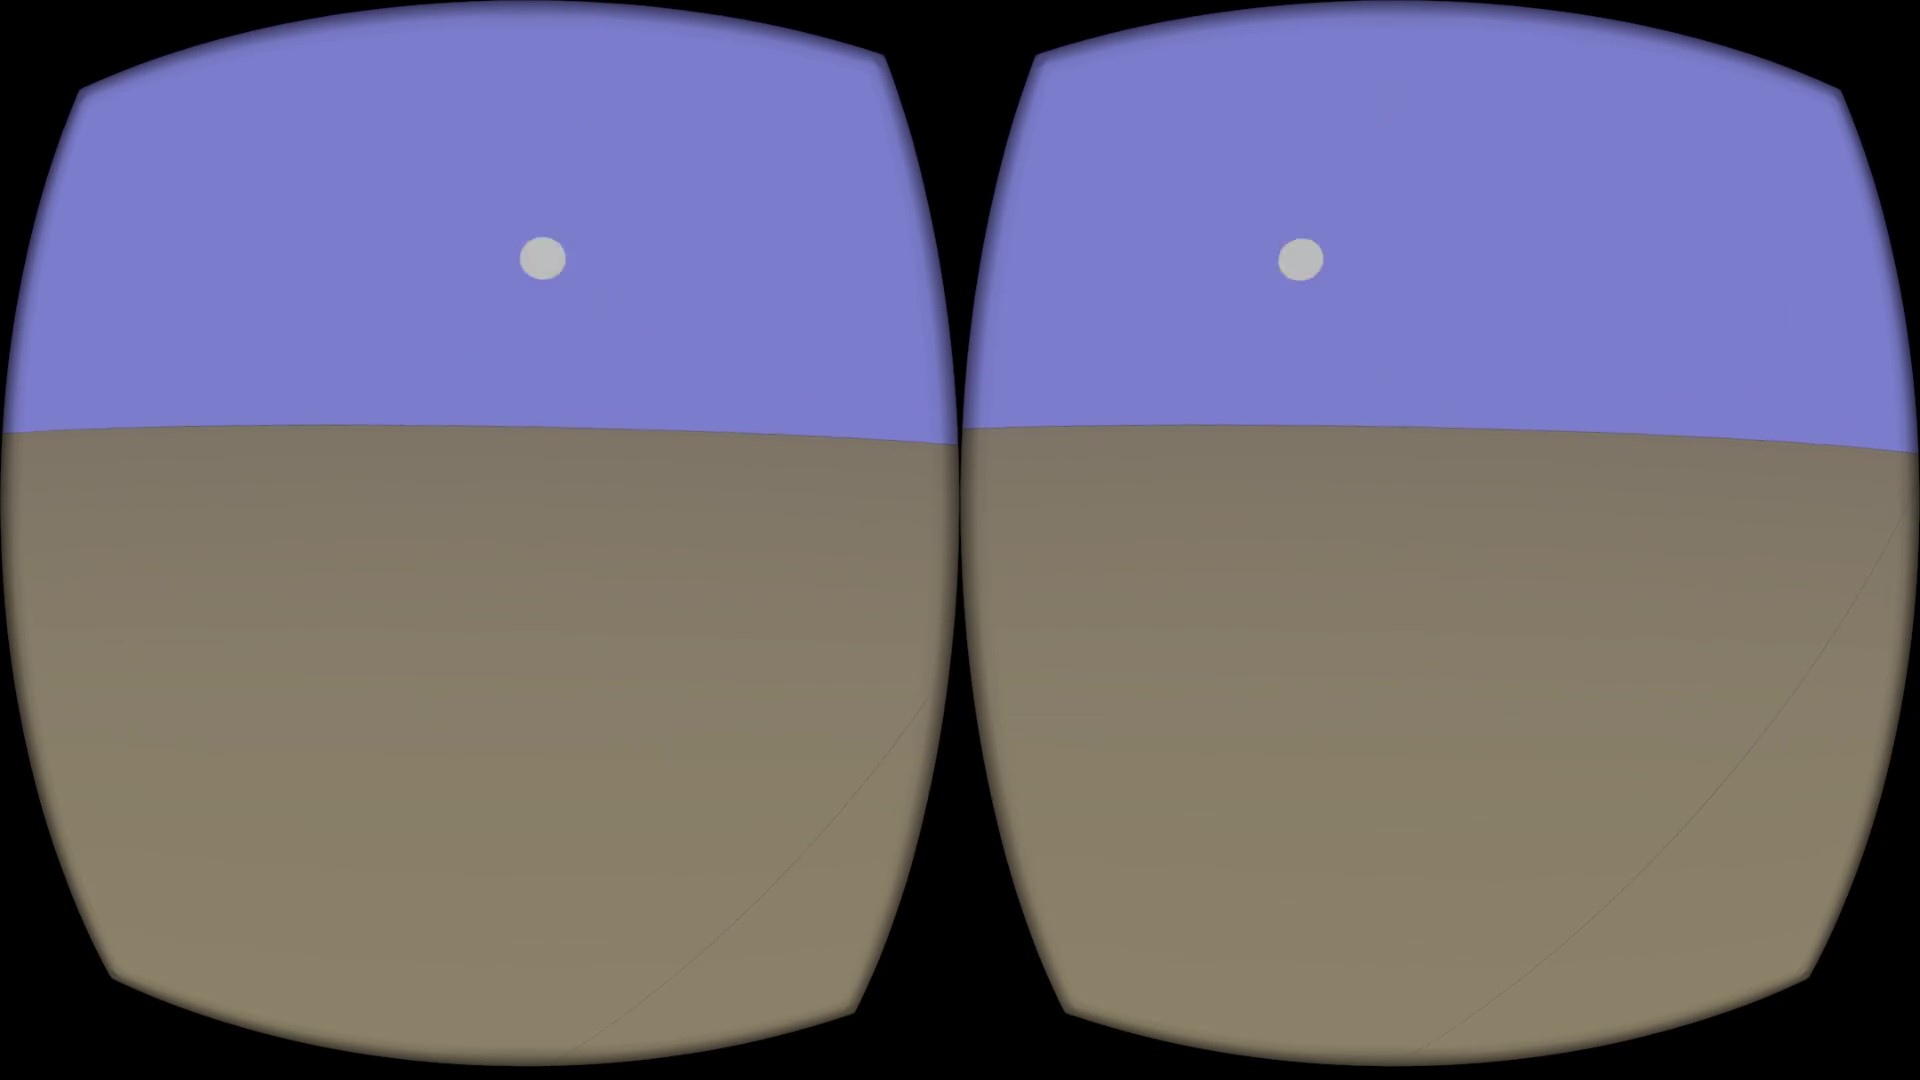
\includegraphics[width=0.45\linewidth]{figures/pre_draw} &
       	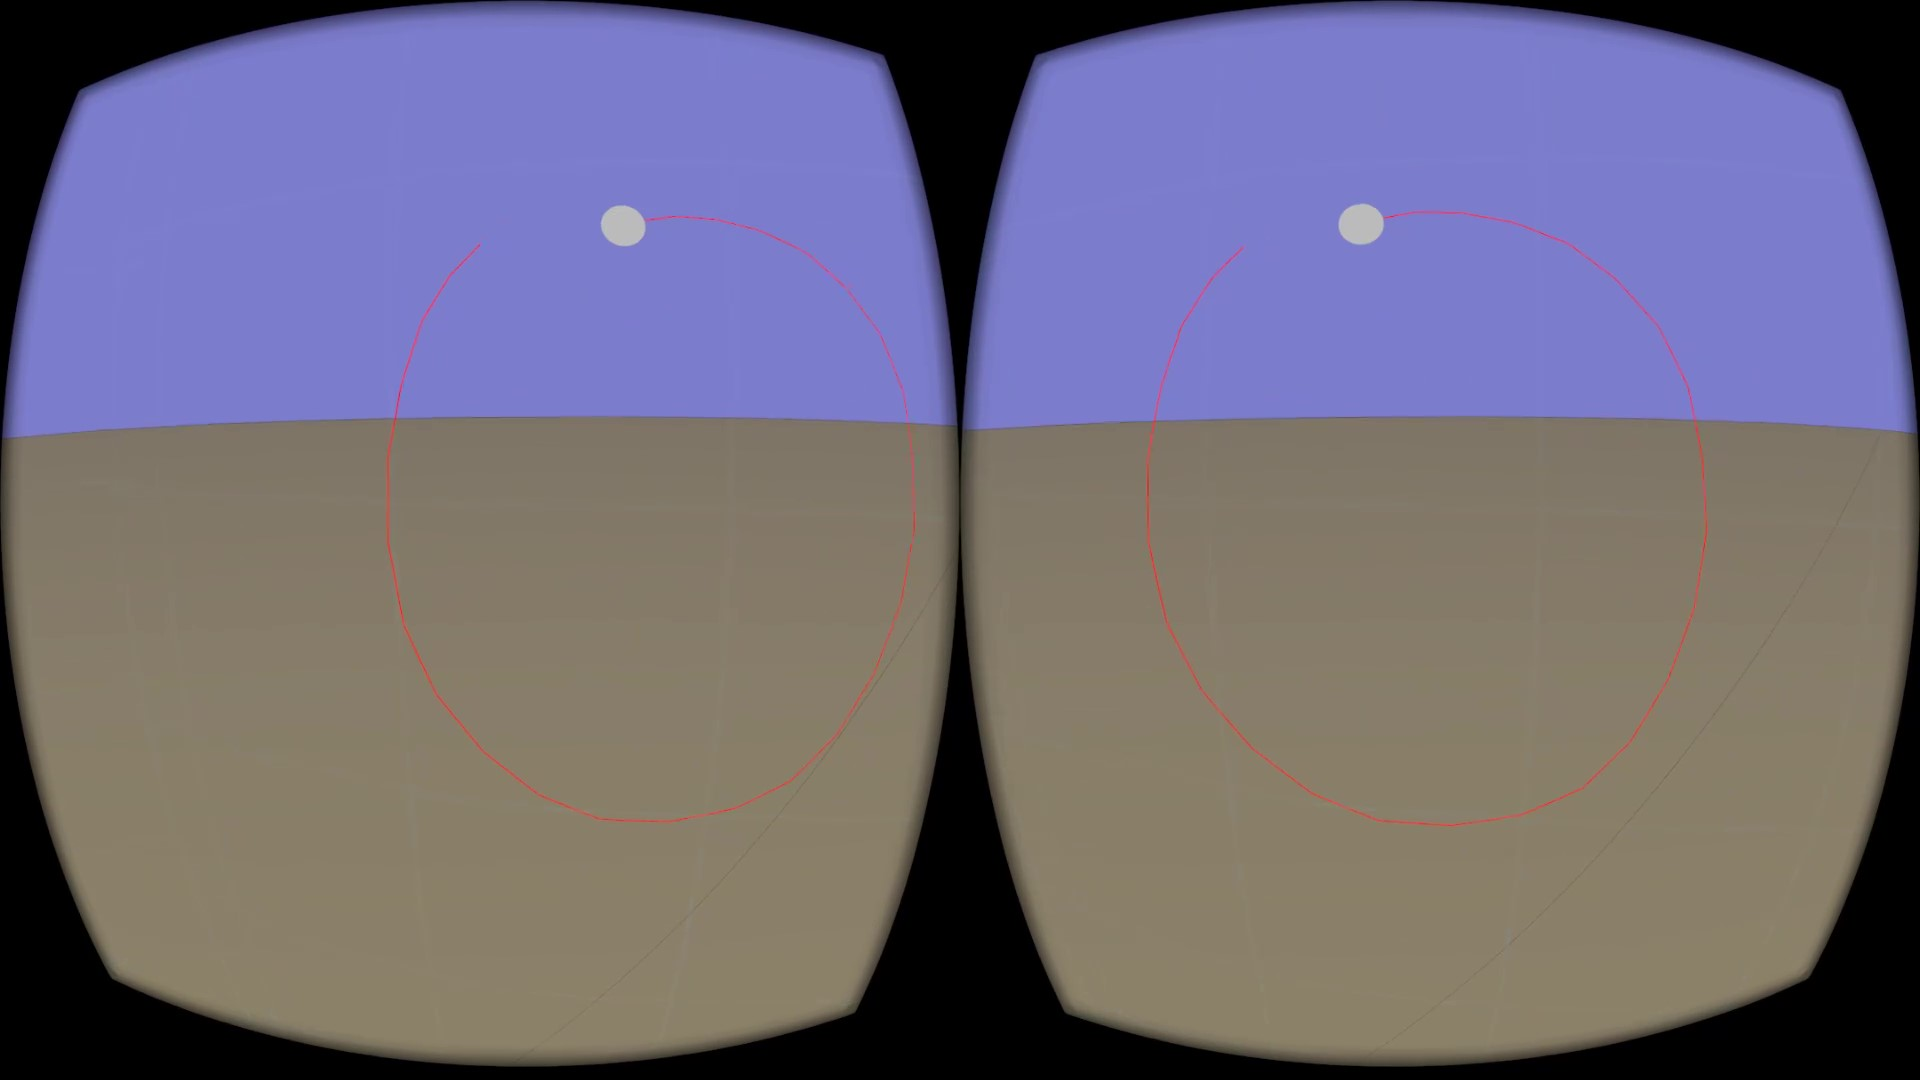
\includegraphics[width=0.45\linewidth]{figures/during_draw} \\
       	(a)&(b)\\
       	\end{tabular}
       	
       	  \centering
    \setlength{\tabcolsep}{0.0130\linewidth}
    \begin{tabular}{@{}c@{}}
    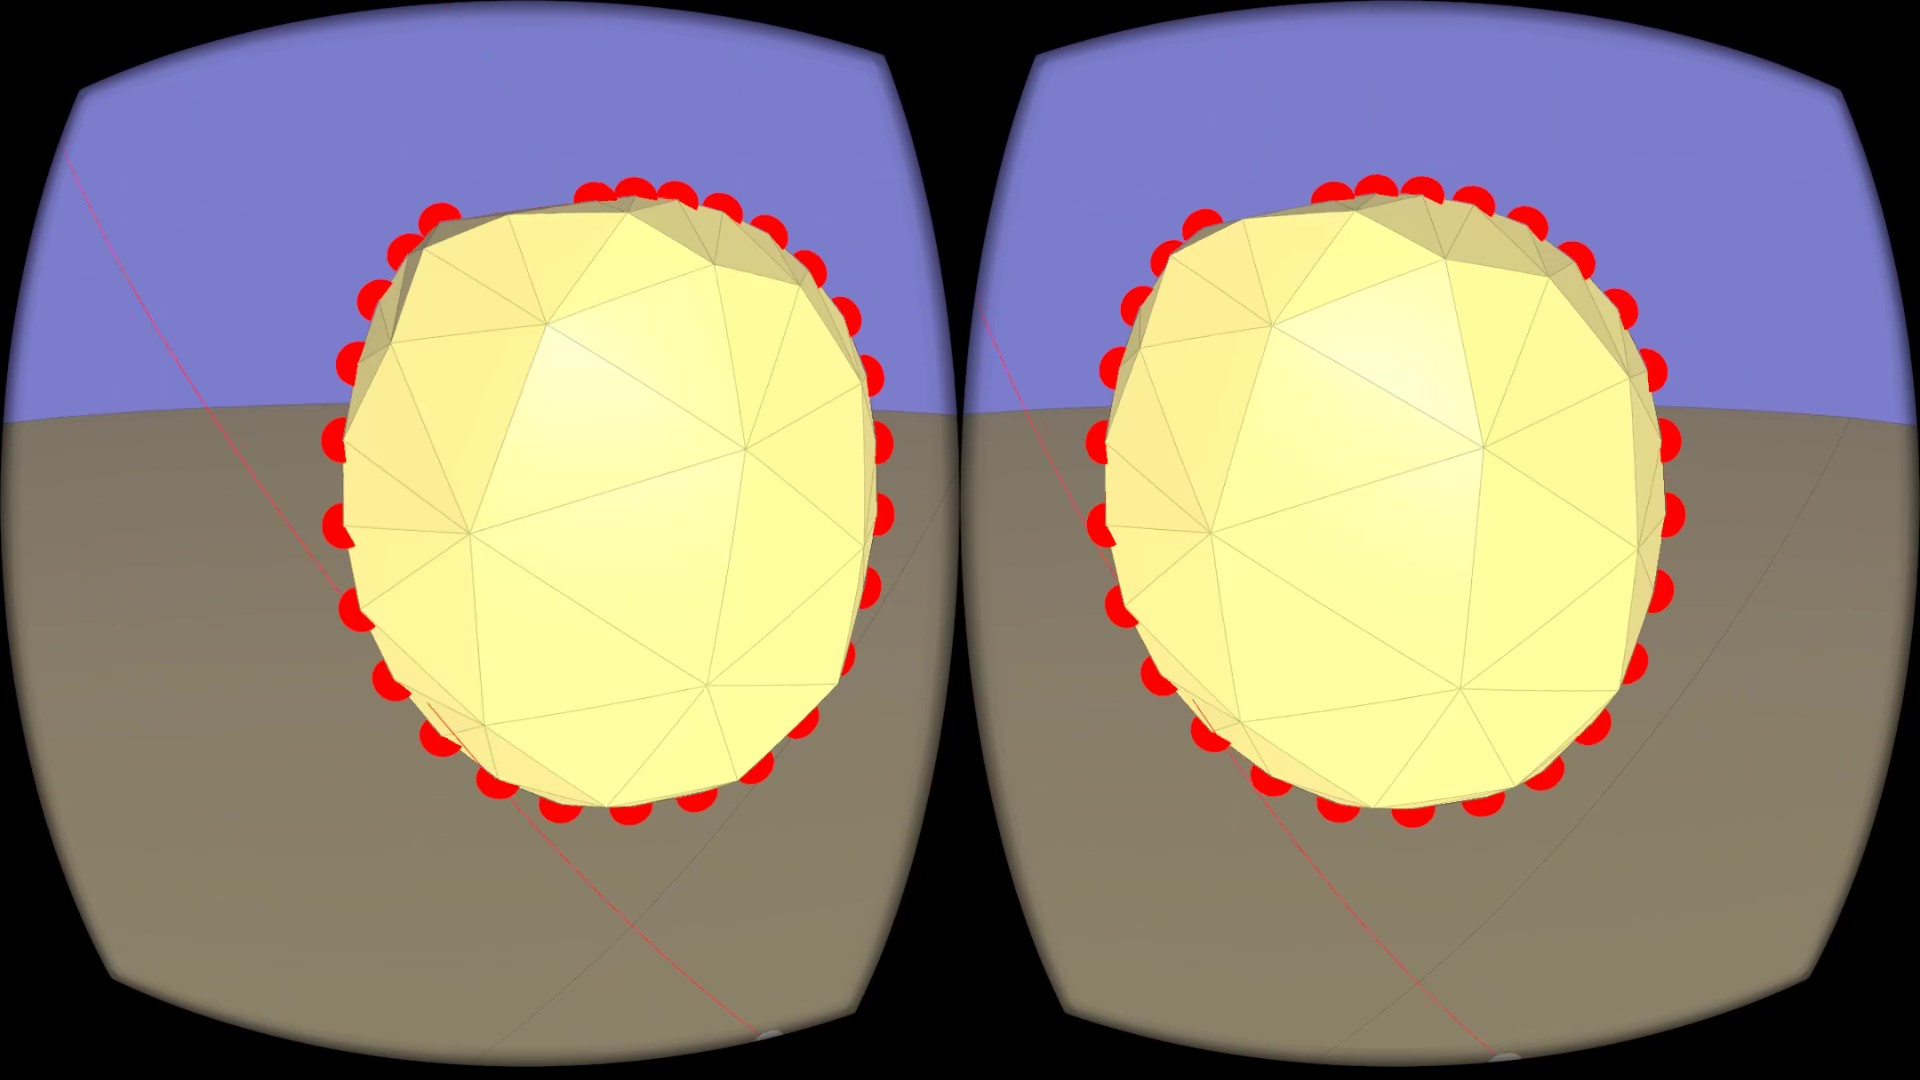
\includegraphics[width=0.926\linewidth]{figures/post_draw}\\
    (c)
    \end{tabular}
    
   
    \caption[Drawing action]{Drawing action.
    	  \textup{(a)} Before \textup{(b)} During \textup{(c)} After
      \label{fig:draw_example}}
\end{figure}

\subsection{Adding and removing control curves}
In the non-VR case, adding control curves on the mesh and later removing them is done by unprojecting the screen coordinates onto the mesh in order to get 3D positions and decide where the user wanted to add/remove a curve. In VR, instead of unprojecting the screen coordinates of the hand or taking the direct hand coordinates, we cast a ray from the hand position in the direction that the controller is being held. This intersection between this ray and the mesh is then used as the final 3D position for adding/removal. Figures~\ref{fig:add_example} and~\ref{fig:remove_example} show what the curve adding and removal actions look like respectively.

\begin{figure}[!h]
    \centering
    \setlength{\tabcolsep}{0.0130\linewidth}
    \begin{tabular}{@{}cc@{}}
    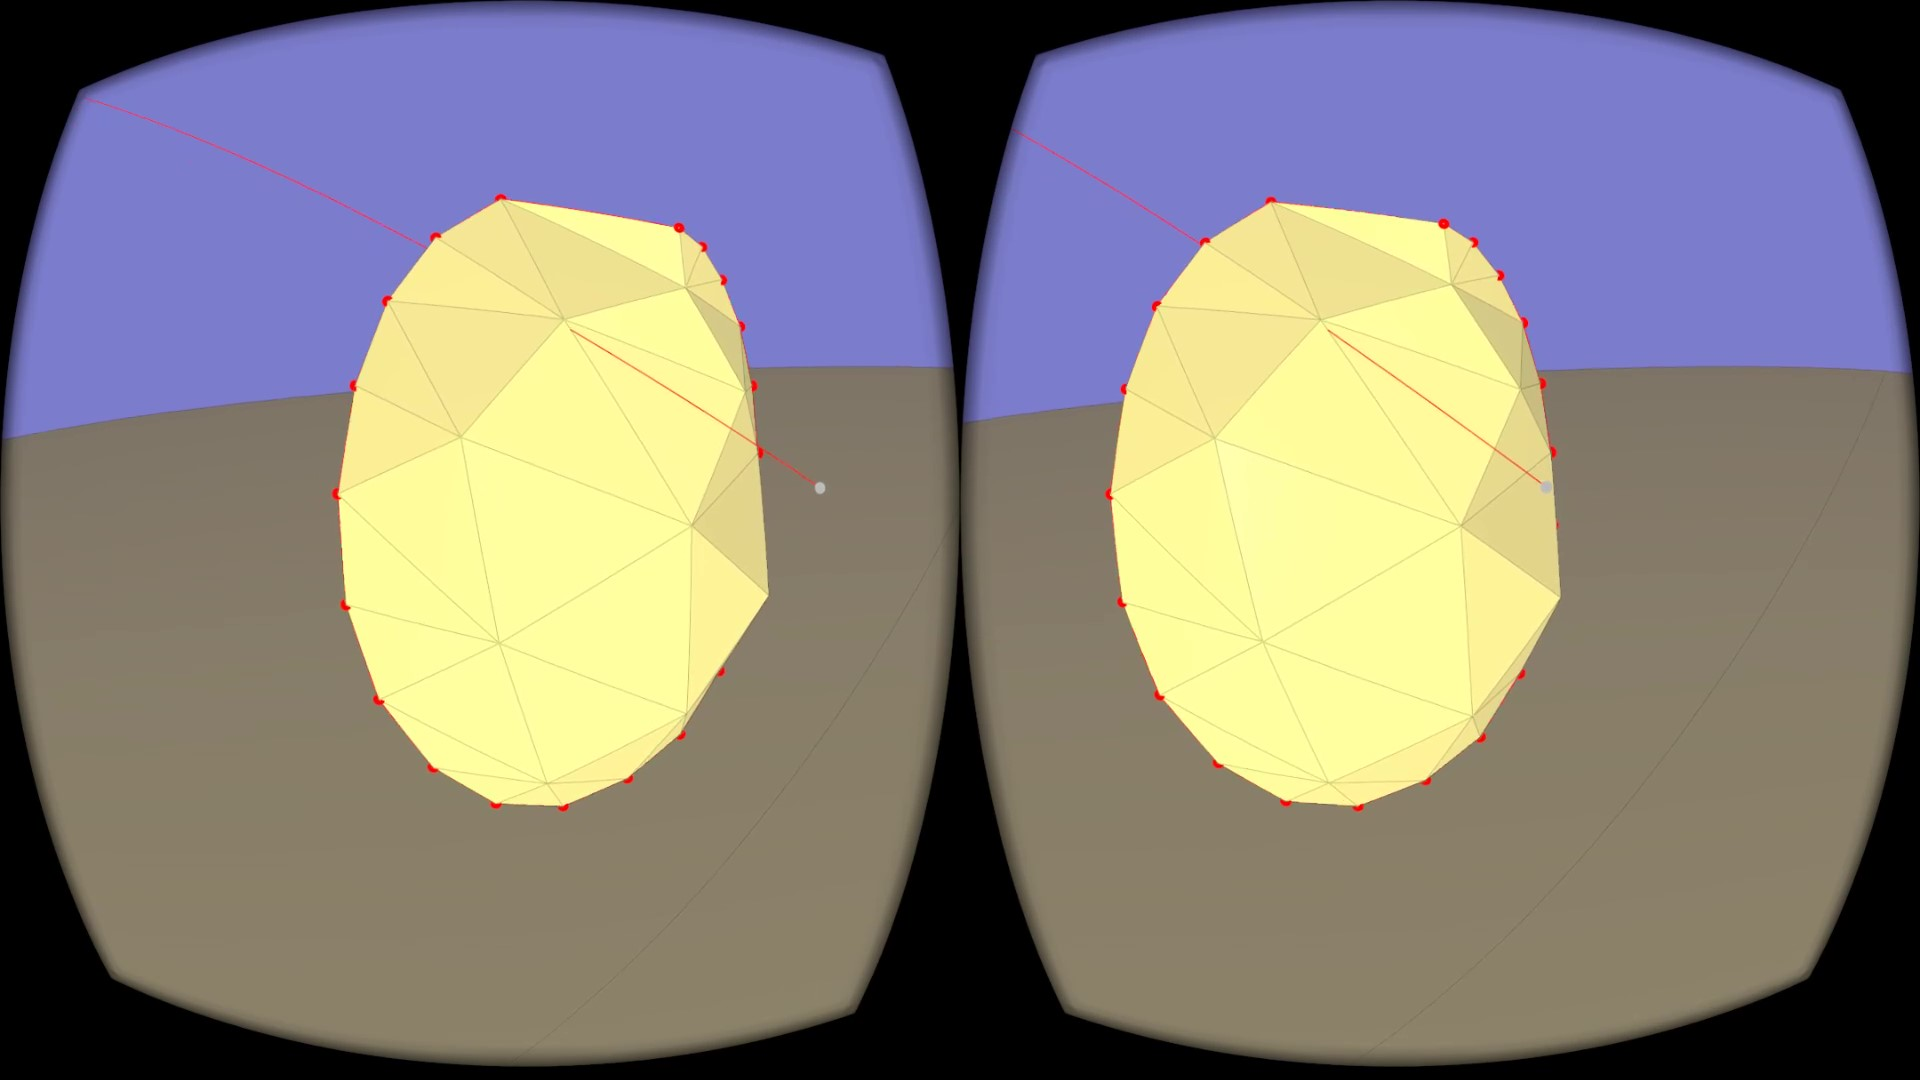
\includegraphics[width=0.45\linewidth]{figures/pre_add} &
       	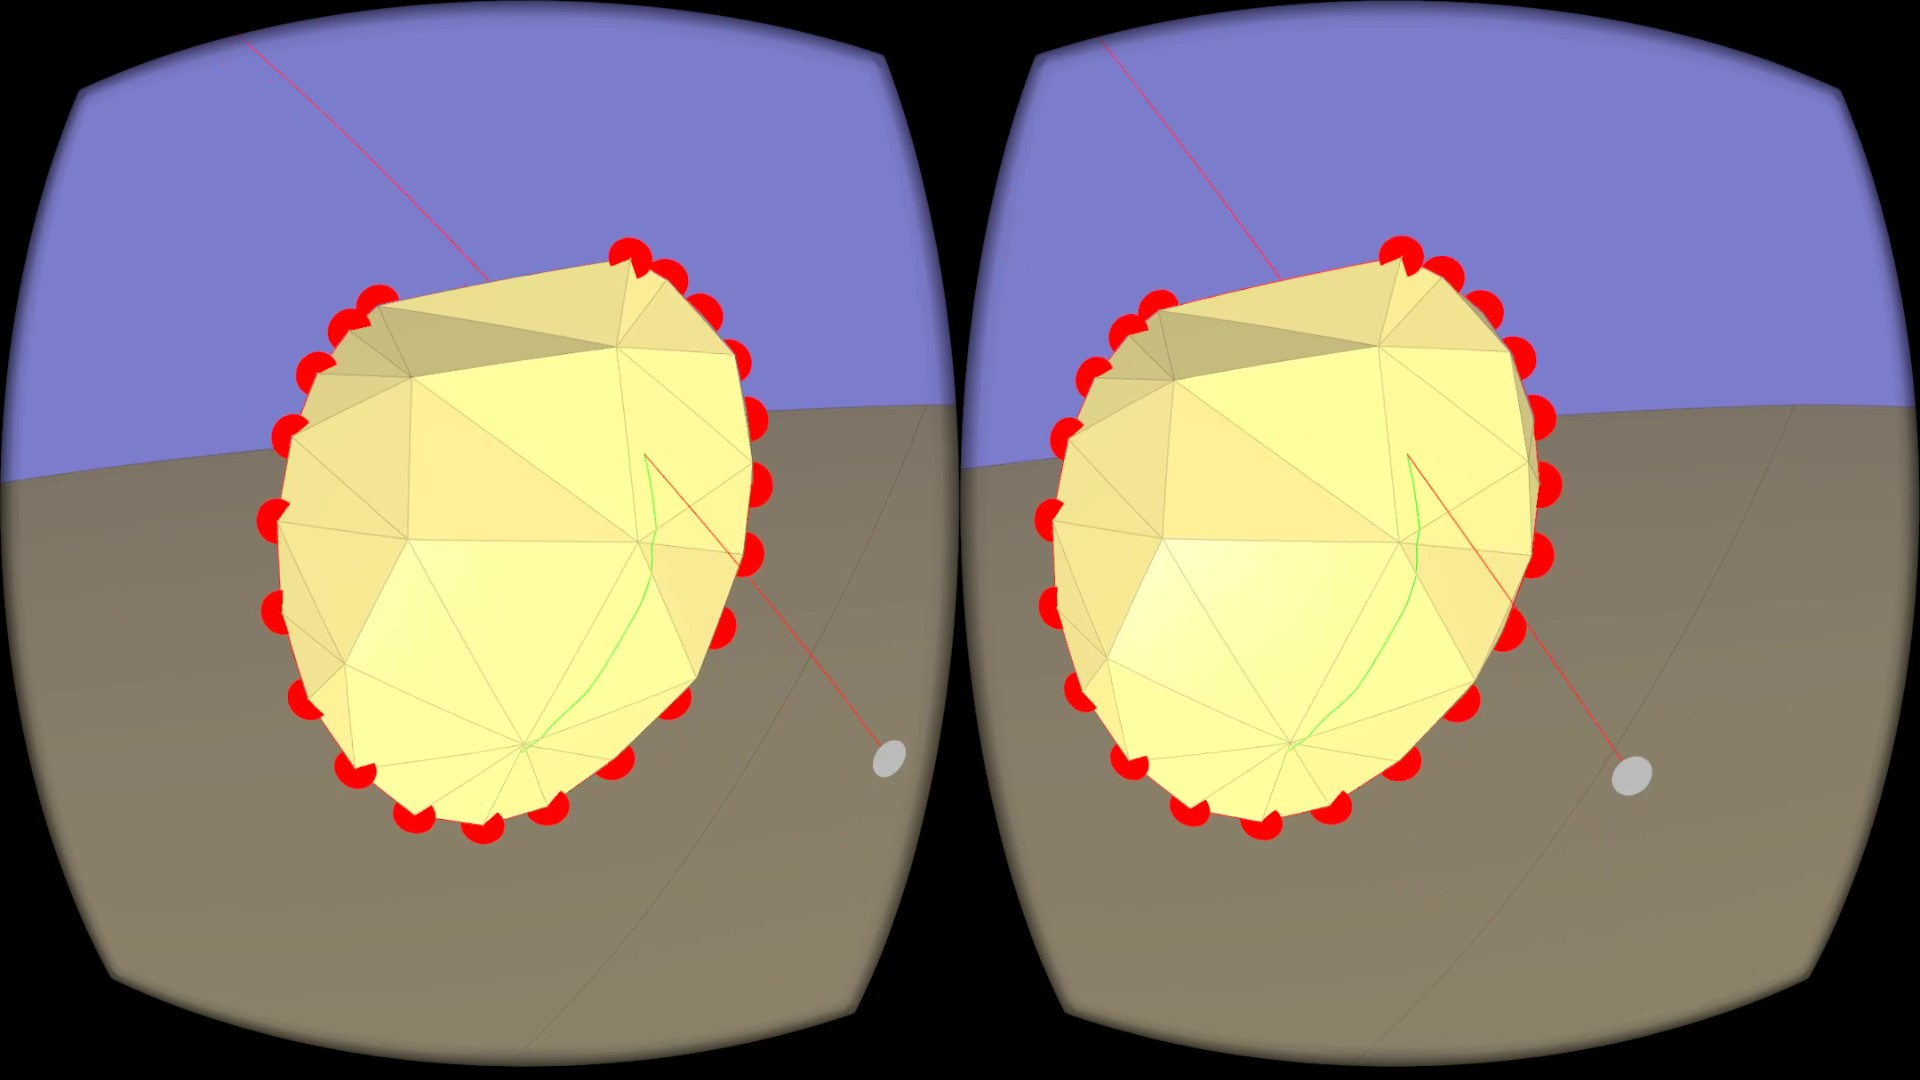
\includegraphics[width=0.45\linewidth]{figures/during_add} \\
       	(a)&(b)\\
       	\end{tabular}
       	
       	  \centering
    \setlength{\tabcolsep}{0.0130\linewidth}
    \begin{tabular}{@{}c@{}}
    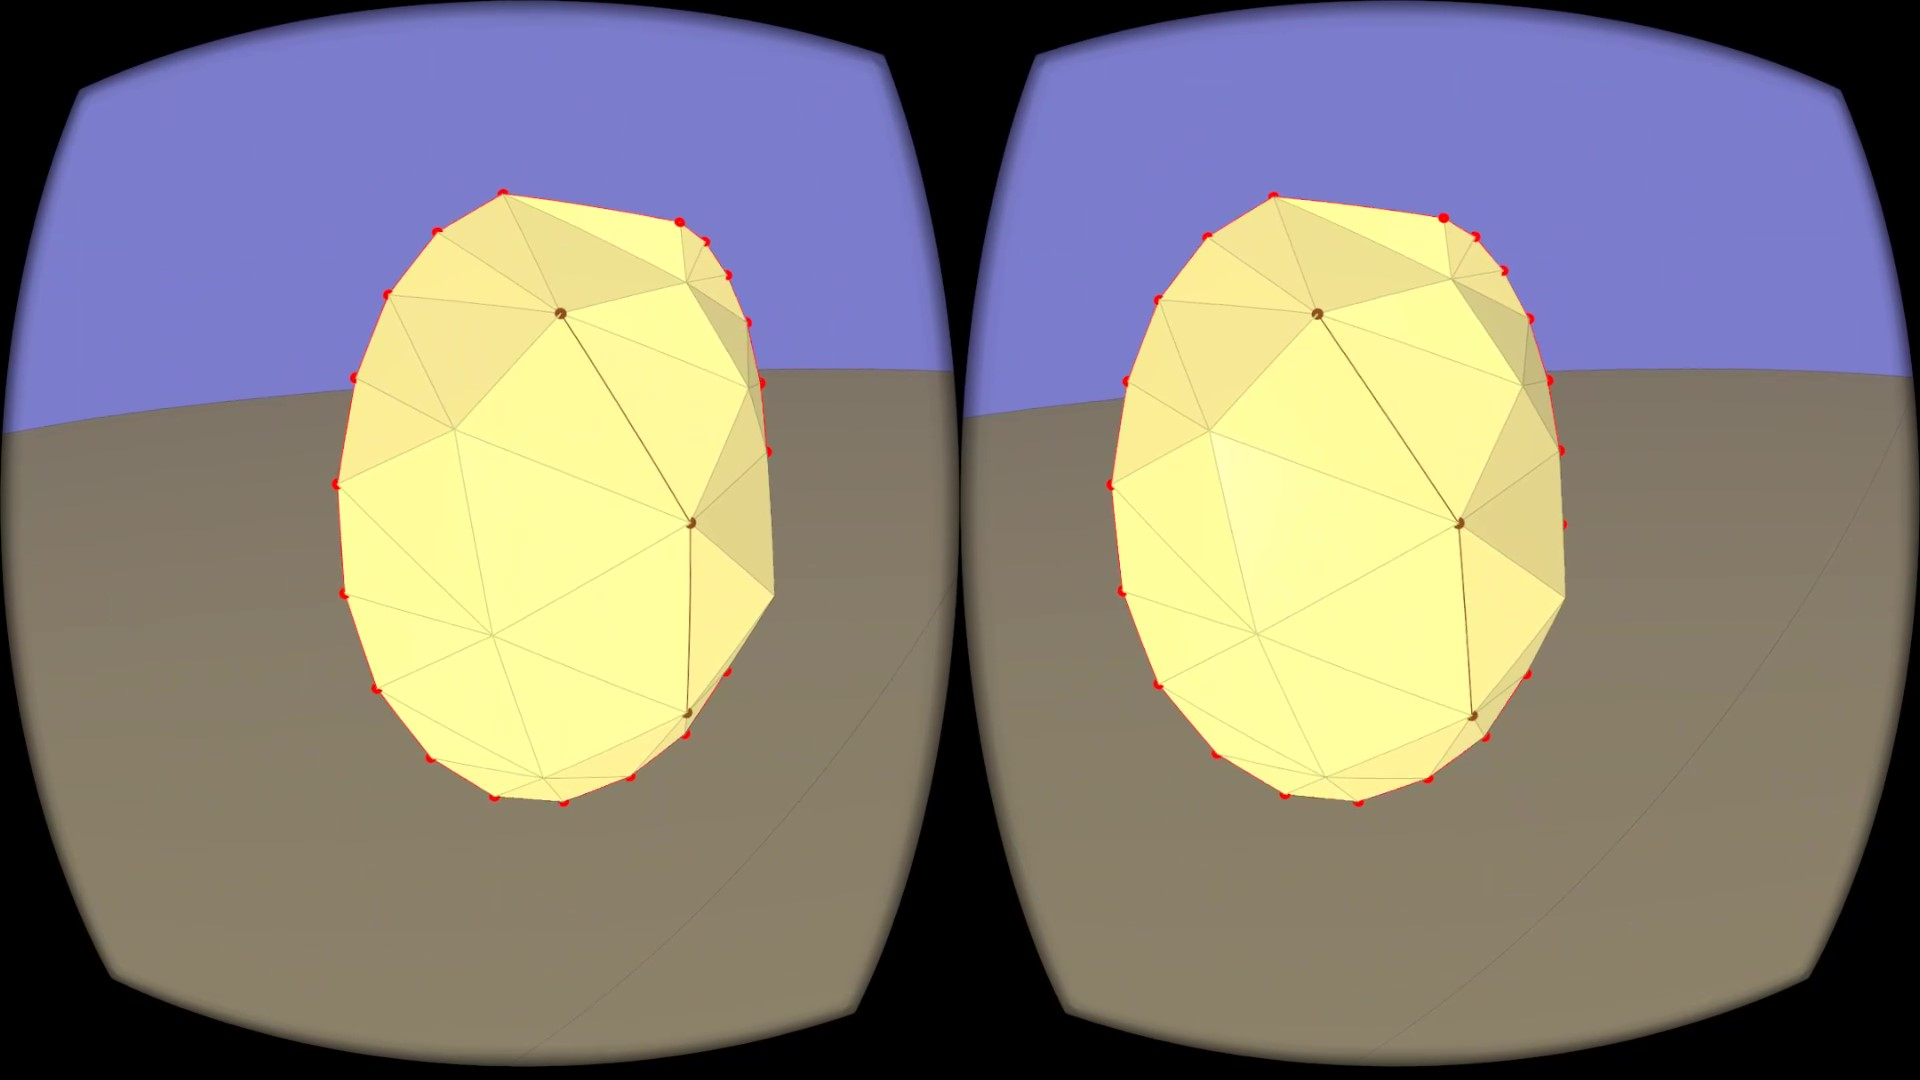
\includegraphics[width=0.926\linewidth]{figures/post_add}\\
    (c)
    \end{tabular}
    \caption[Curve adding action]{Curve adding action.
    	  \textup{(a)} Before \textup{(b)} During \textup{(c)} After
      \label{fig:add_example}}
\end{figure}

\begin{figure}[!h]
    \centering
    \setlength{\tabcolsep}{0.0130\linewidth}
    \begin{tabular}{@{}cc@{}}
    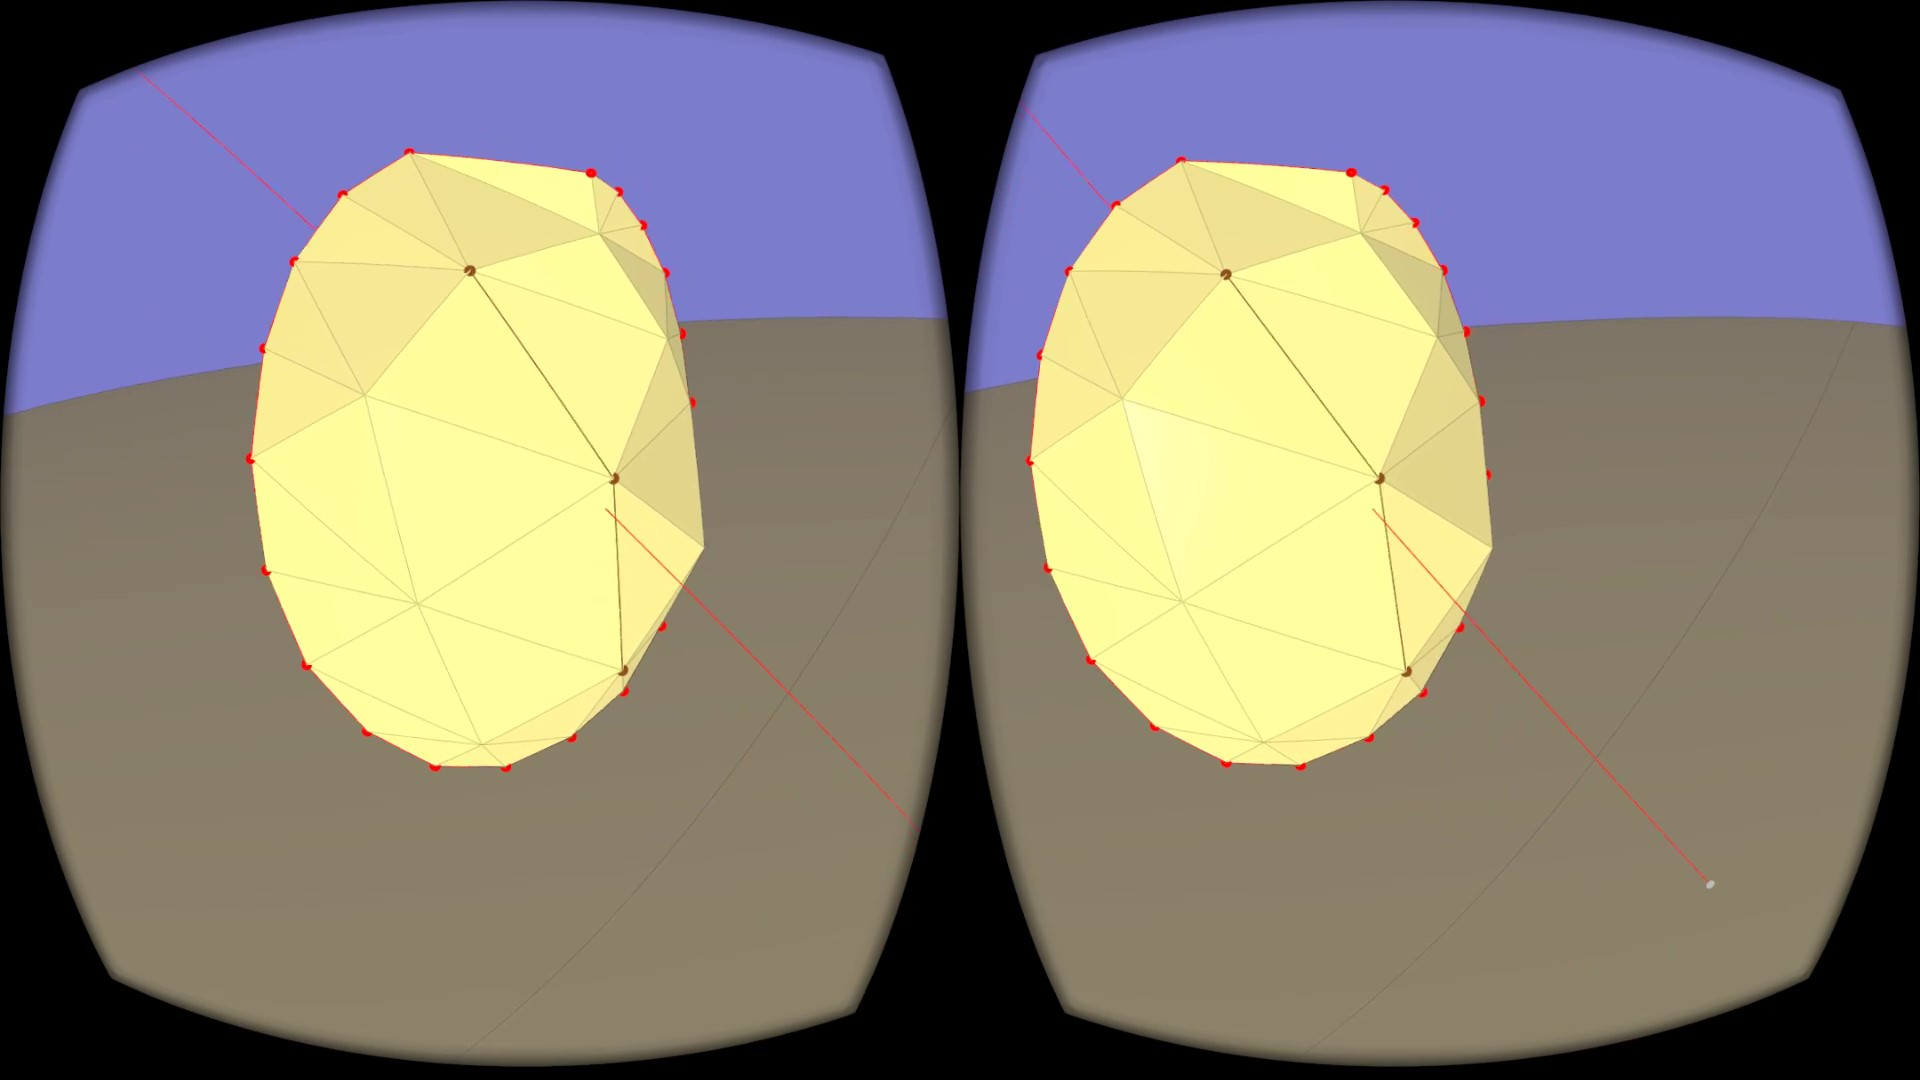
\includegraphics[width=0.45\linewidth]{figures/pre_remove} &
       	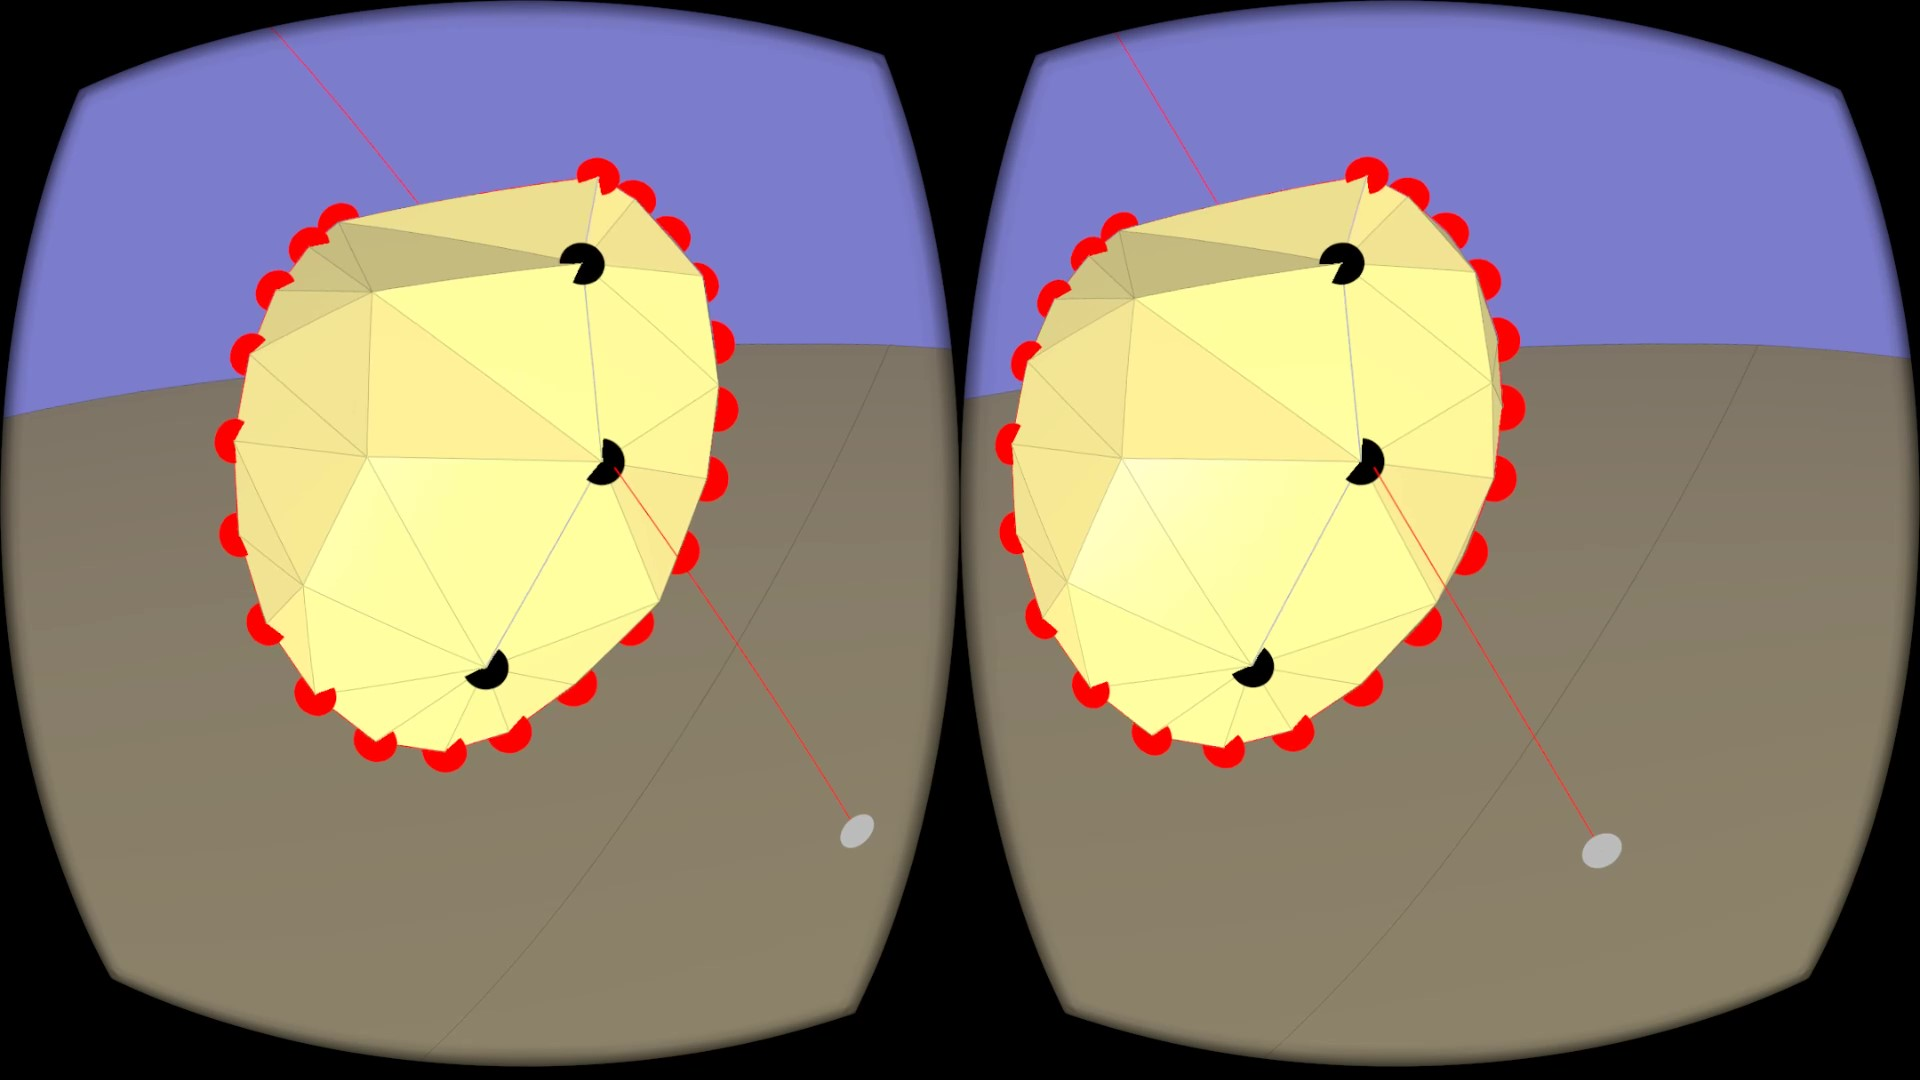
\includegraphics[width=0.45\linewidth]{figures/during_remove} \\
       	(a)&(b)\\
       	\end{tabular}
       	
       	  \centering
    \setlength{\tabcolsep}{0.0130\linewidth}
    \begin{tabular}{@{}c@{}}
    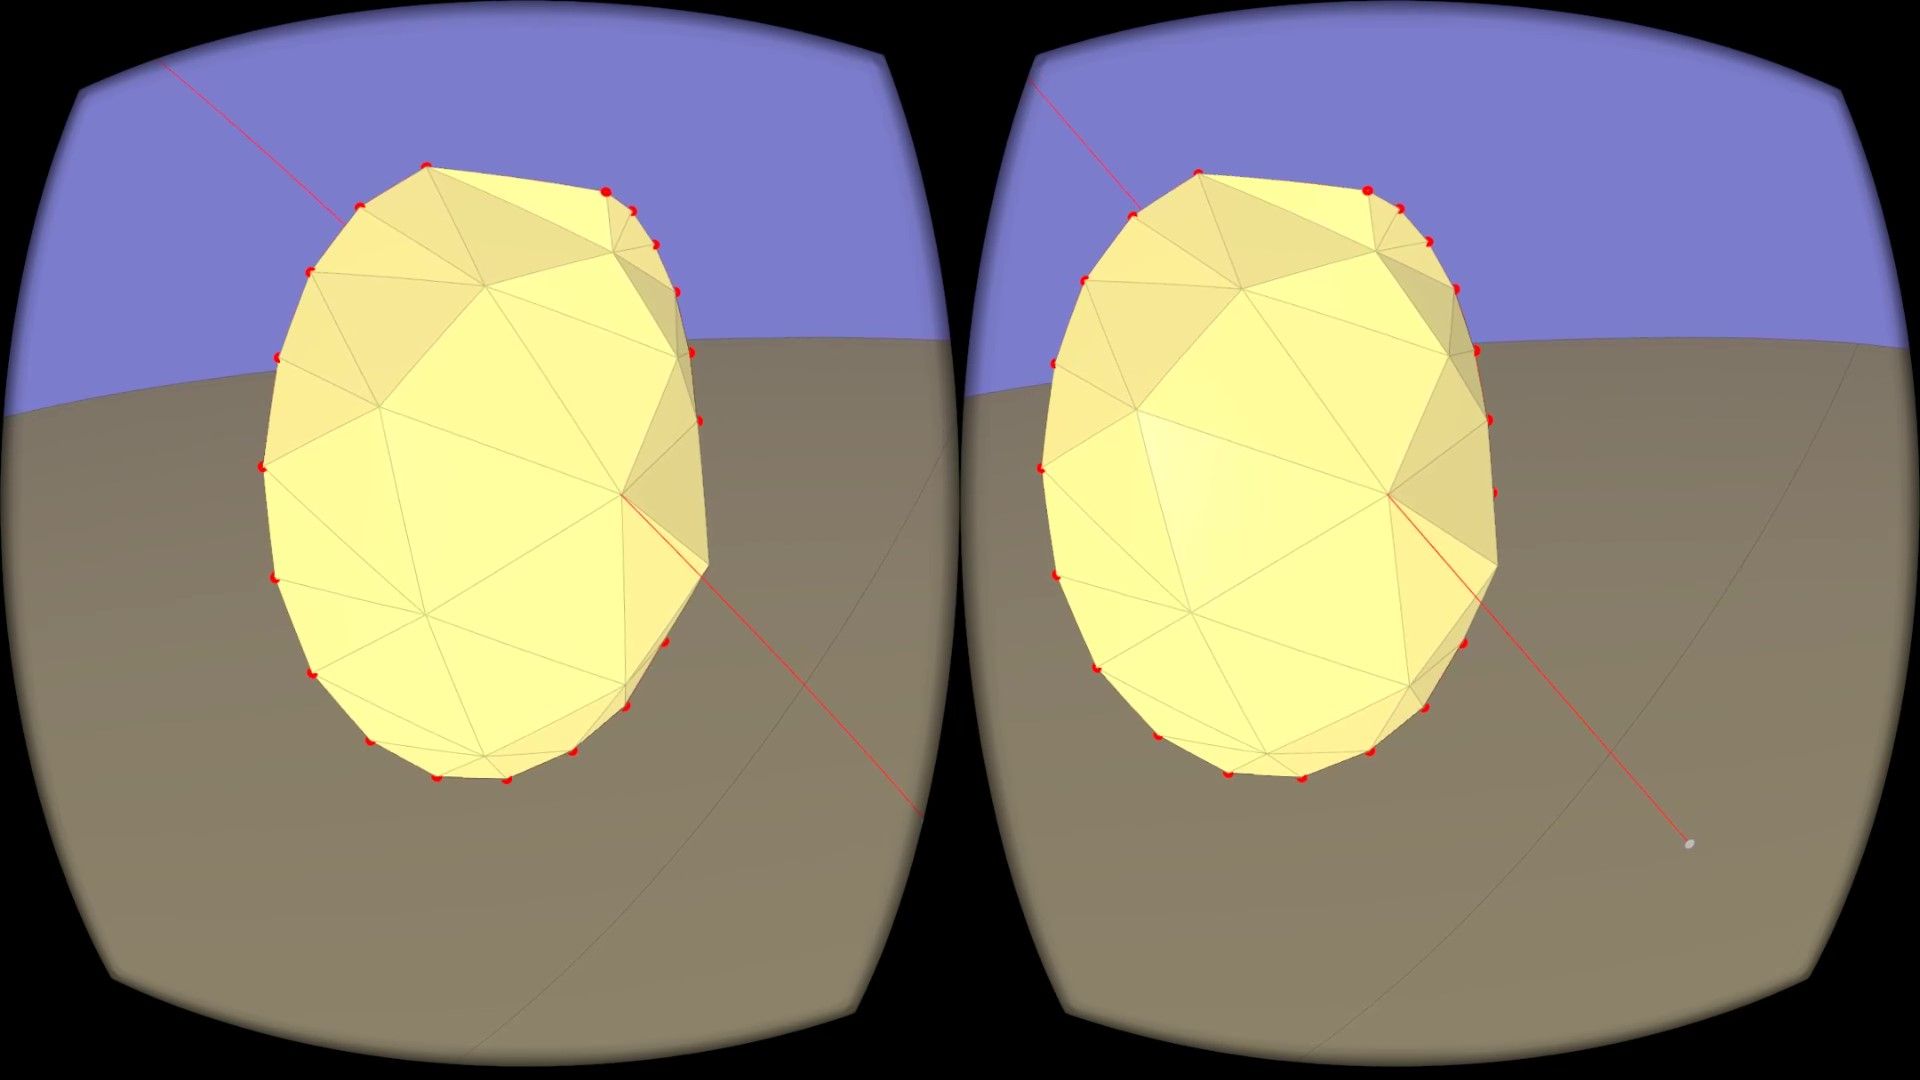
\includegraphics[width=0.926\linewidth]{figures/post_remove}\\
    (c)
    \end{tabular}
    
   
    \caption[Stroke removal action]{Stroke removal action.
    	  \textup{(a)} Before \textup{(b)} During \textup{(c)} After
      \label{fig:remove_example}}
\end{figure}

\subsection{Cutting}
When cutting in the non-VR program, the drawn stroke is interpreted purely in 2D screen coordinates. In order to create a loop on the front and back of the mesh surface, the algorithm checks which edges are crossed (in 2D) by a line segment between two consecutive stroke points. Since the same 2D points are used for creating a surface path on the backside of the mesh, this results in perpendicular cuts (meaning that the "cutting knife" always goes perpendicular through the screen, and never at an angle). On the other hand, when cutting in VR we take the coordinates of both the first (front side) and second (back side) intersection between the cutting ray and the mesh. By doing this, we enable the possibility for the user to cut the mesh diagonally, without first having to rotate the mesh. 

In order to check which edges are crossed by the stroke segments, we initially check if the next stroke point lies either in the current polygon or in one of the adjacent ones. If this is not the case, we additionally check for intersections between the edges of the current point's polygon and the plane that is formed by the two points that make up the stroke segment and the position of the hand at the time of drawing that stroke segment. We define the edges in the parametric form of a line and find the value $t$ along the line where it is intersected by the plane. If an edge is intersected with $ 0.01 \leq t \leq 0.99$ (discarding 1\% of the edge length on each side due to numerical imprecision), we know that the stroke segment crosses that edge.

One problem that arises due to the fact that we are using 3D intersection points between the cutting ray and the mesh, is that we cannot easily derive the start and end points of the cutting stroke. These points are the final point outside of the mesh before we start drawing on top of the mesh and the first point outside of the mesh after drawing on top of the mesh respectively. We need these points in order to be able to find the mesh boundary edges that we need to cross to wrap the surface path around to the backside of the mesh. As mentioned before, in the non-VR case we simply use 2D coordinates based off the screen coordinates of the mouse pointer. In VR we cannot take the position of the controller as the user is likely cutting from a distance. 

What we have done in order to determine the start and end point is storing the controller position and direction for a start and end point. The start point is updated with every sampled point that does not intersect the mesh that is sampled before we have started going over the mesh. The end point is updated with every sampled point that does not intersect the mesh and is drawn after we have been on the mesh before. Then when the user releases the controller buttons after drawing the cut stroke, we take these positions and directions and along their resulting rays find the two points that are closest to the first and last point drawn onto the mesh. The two black points in Figure~\ref{fig:schematiccut} represent the start and end point. 

A problem that might arise when the user draws the cut stroke too fast (resulting in larger distances between the sampled stroke points) is that the algorithm fails to create a closed surface path over the mesh. This can happen when the resulting stroke points have at least one empty polygon between them, and the plane that is spanned by the two subsequent stroke points and the position of the controller at the time of drawing intersects the edge outside of the allowed range ($t \leq 0.01$ or $t \geq 0.99$). As a result of this, the algorithm is not be able to find an edge to cross in order to move in the direction of the next stroke point and gets stuck. If this happens, a beep will sound and the cut stroke will be drawn in black, similar to what is shown in Figure~\ref{fig:errordisplay}. Figure~\ref{fig:schematiccut} gives a schematic overview of the problem that might arise with a cut stroke.

\begin{figure}[!h]
    \centering
    \setlength{\tabcolsep}{0.0130\linewidth}
    \begin{tabular}{@{}cc@{}}
    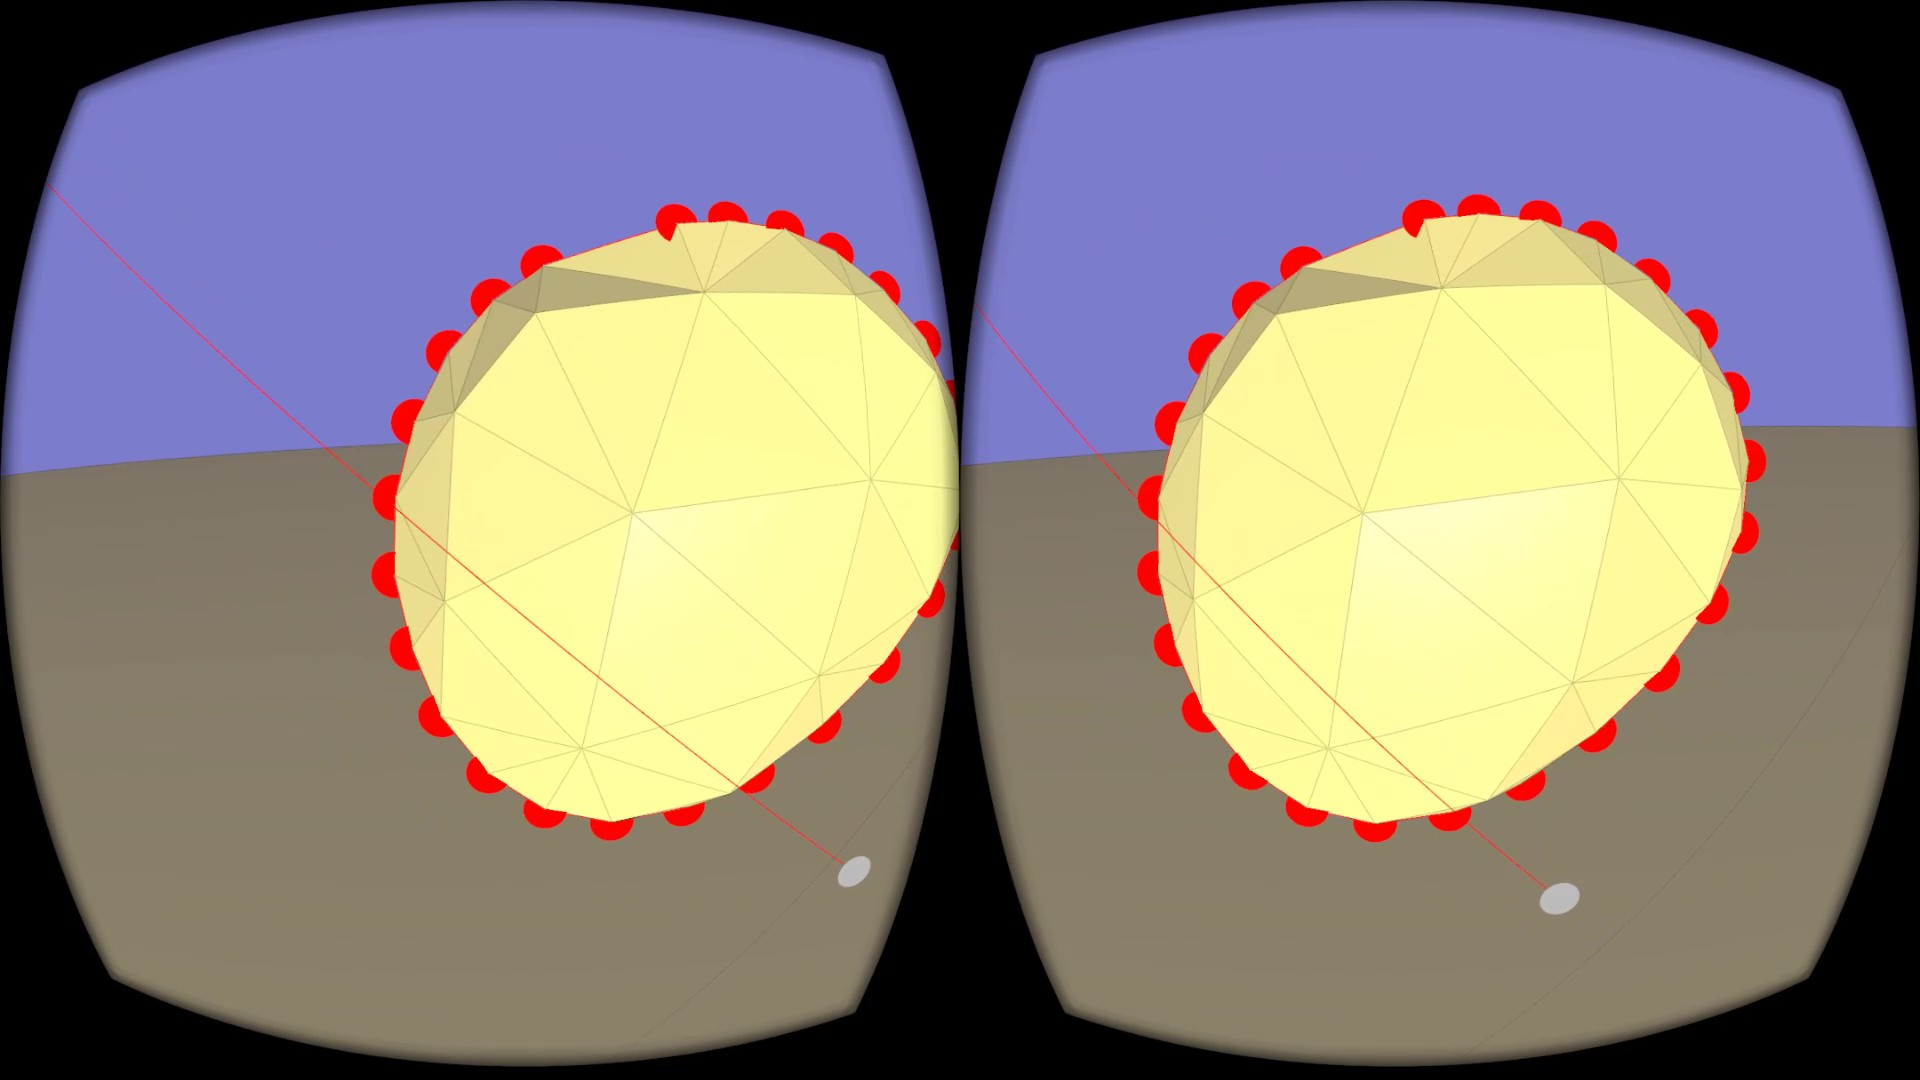
\includegraphics[width=0.45\linewidth]{figures/pre_cut} &
       	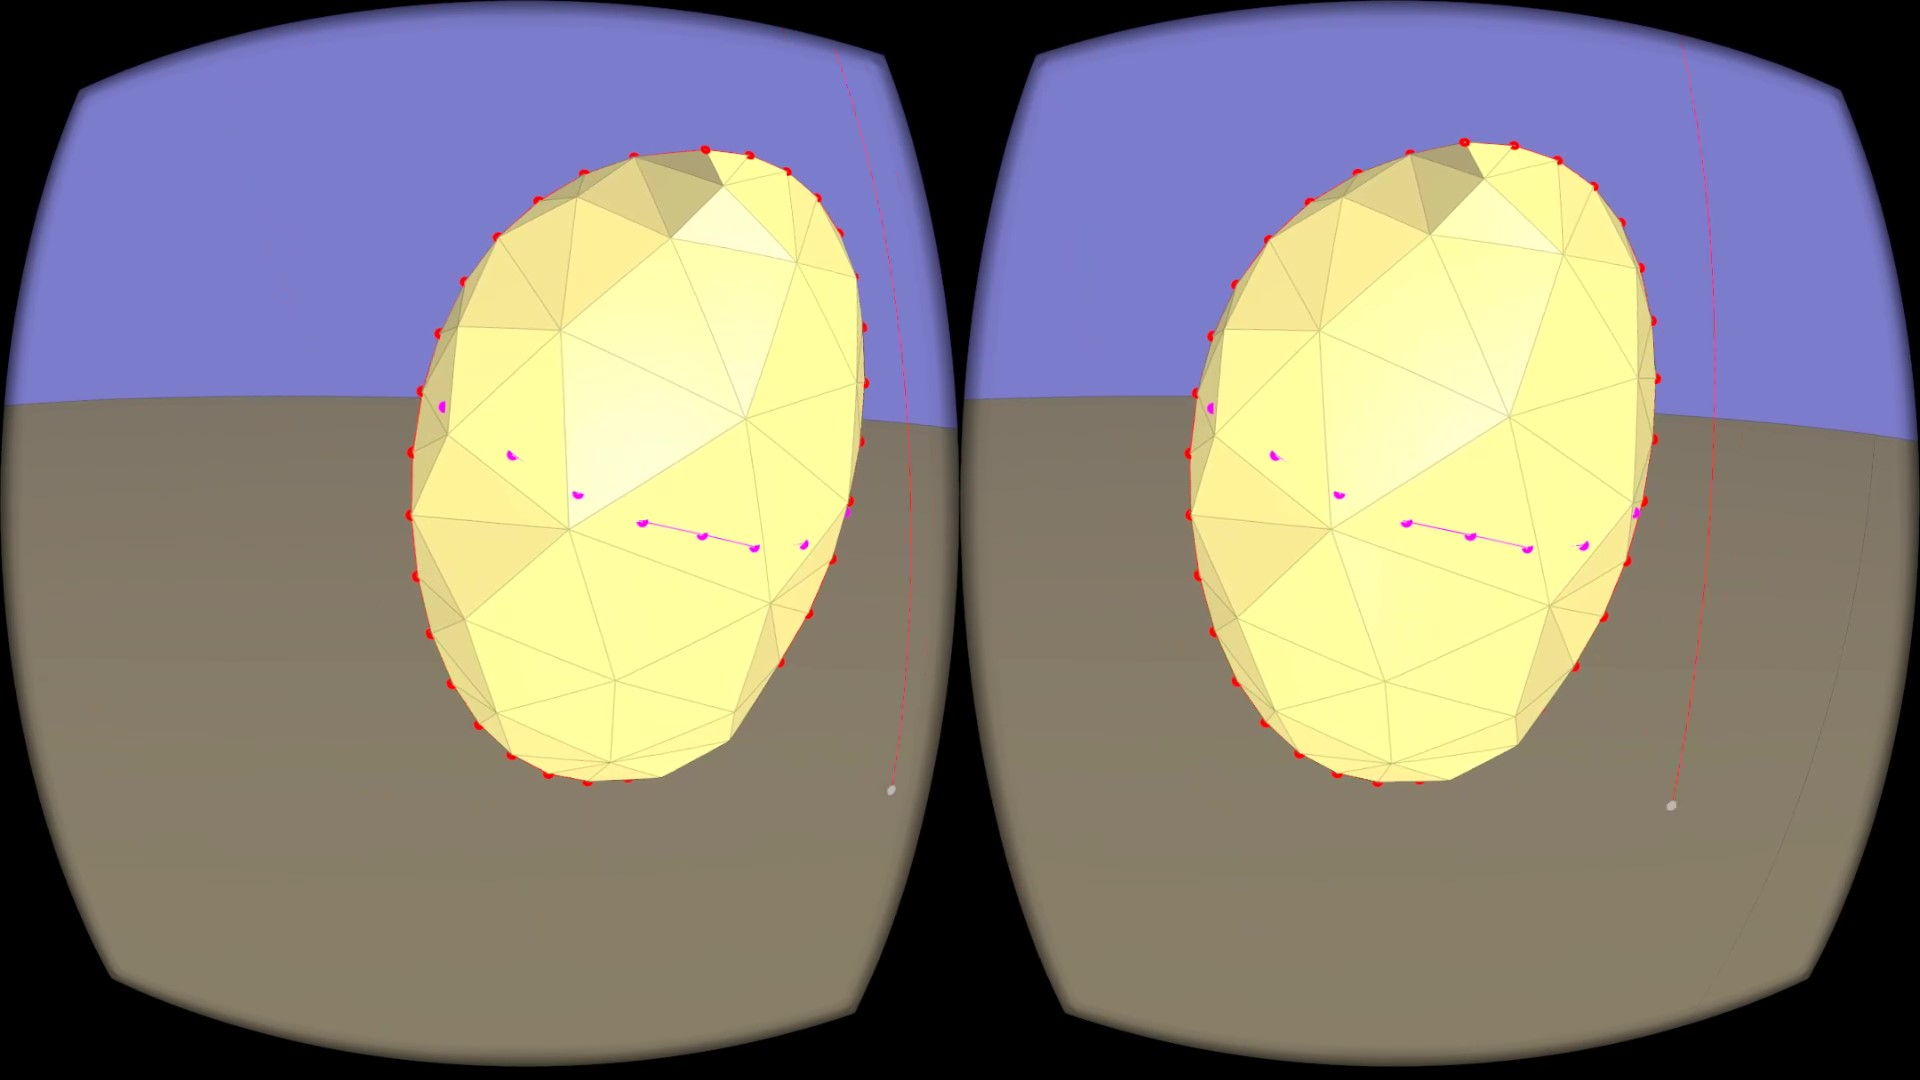
\includegraphics[width=0.45\linewidth]{figures/during_cut} \\
       	(a)&(b)\\
       	\end{tabular}
       	
       	  \centering
    \setlength{\tabcolsep}{0.0130\linewidth}
    \begin{tabular}{@{}c@{}}
    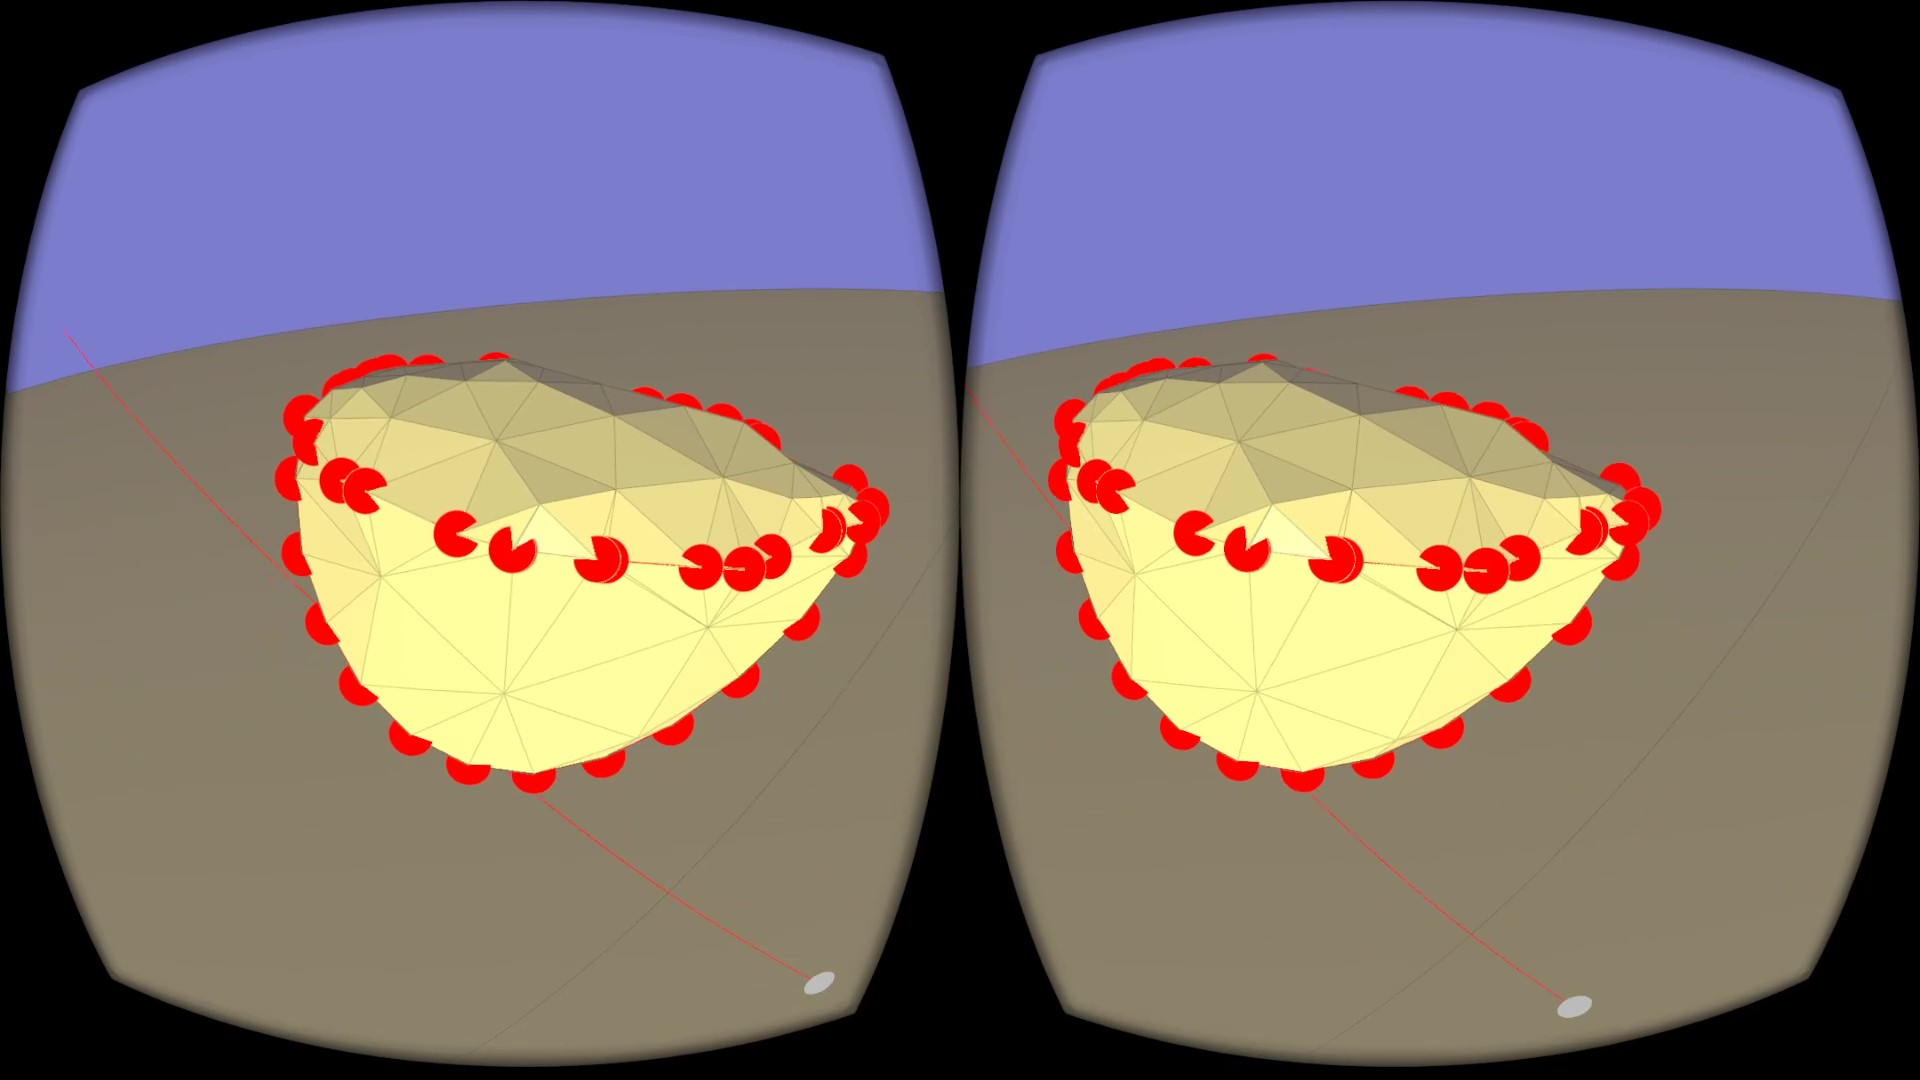
\includegraphics[width=0.926\linewidth]{figures/post_cut}\\
    (c)
    \end{tabular}
    \caption[Cutting action]{Cutting action.
    	  \textup{(a)} Before \textup{(b)} During \textup{(c)} After
      \label{fig:cut_example}}
\end{figure}

\begin{figure}[!h]
    \centering
    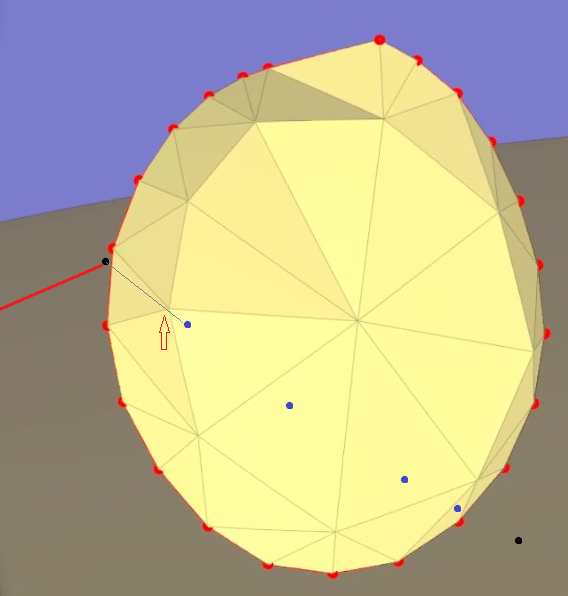
\includegraphics[width=0.5\linewidth]{figures/schematic_error_cut1}\\
    \caption[Schematic drawing of a problematic cut]{Schematic drawing of a problematic cut stroke. The black off-mesh point and the left-most on-mesh point are separated by an empty polygon. The intersection with the edge that is indicated with the red arrow is discarded due to being out of range.
      \label{fig:schematiccut}}
\end{figure}

\subsection{Extrusion}
The surface path for the extrusion base is created in a similar fashion to the cutting path, except that only the first hit between ray and mesh (front side intersection) is used. Drawing the extrusion silhouette in VR is significantly different from the way it is done in non-VR. When defining the silhouette stroke in non-VR, the user first has to rotate the mesh such that it is shown from a side view. Only then can the user sensefully specify the shape and depth of the extrusion silhouette, since we cannot specify any depth information from a frontal view of the extrusion base. The z-value of the silhouette stroke in this view is determined by projecting the silhouette stroke points onto one of the normal planes of the extrusion base. We select the plane that goes through the "left-most" (point with the smallest projected value onto a axis perpendicular to the base normal) silhouette base vertex, which means that the silhouette points will lie in a line between the left-most and right-most base vertex. 
In VR on the other hand, we know the actual 3D positions of the controller and can therefore directly specify the extrusion silhouette in a frontal view of the extrusion base. If the user prefers to do this from a side view instead (to get additional visual feedback about the silhouette depth on top of the tactile feedback), this is also possible. 

However, because the user also has control over the z-coordinate, the silhouette stroke is no longer guaranteed to lie on a line between the "left-most" and "right-most" base stroke points. This can give problems when projecting the silhouette points to 2D in preparation for triangulation. For the purpose of triangulation, the base stroke is divided in a left and right part, and together with the silhouette stroke each of these forms a half-dome. Both of these half domes are projected to 2D and then individually triangulated, unprojected back to 3D and finally stitched to each other. Because the silhouette is no longer guaranteed to lie on a straight line, it can happen that when we project the two half-domes onto the plane perpendicular to the base stroke normal, some of the silhouette points project to the wrong side of the base stroke points that complete the half-dome. Triangulating such a projection where the silhouette points flipped over to the other side will results in holes in the mesh. To overcome this problem, we project the points of each half-dome loop onto the plane that is perpendicular to the normals of each individual half-dome. This prevents the silhouette stroke points from projecting to the wrong side of the extrusion base stroke and thus will avoid meshes with holes. Figure~\ref{fig:extrude_example} shows the mesh pre, during and post a successful extrusion operation.

\begin{figure}[!h]
    \centering
    \setlength{\tabcolsep}{0.0130\linewidth}
    \begin{tabular}{@{}cc@{}}
    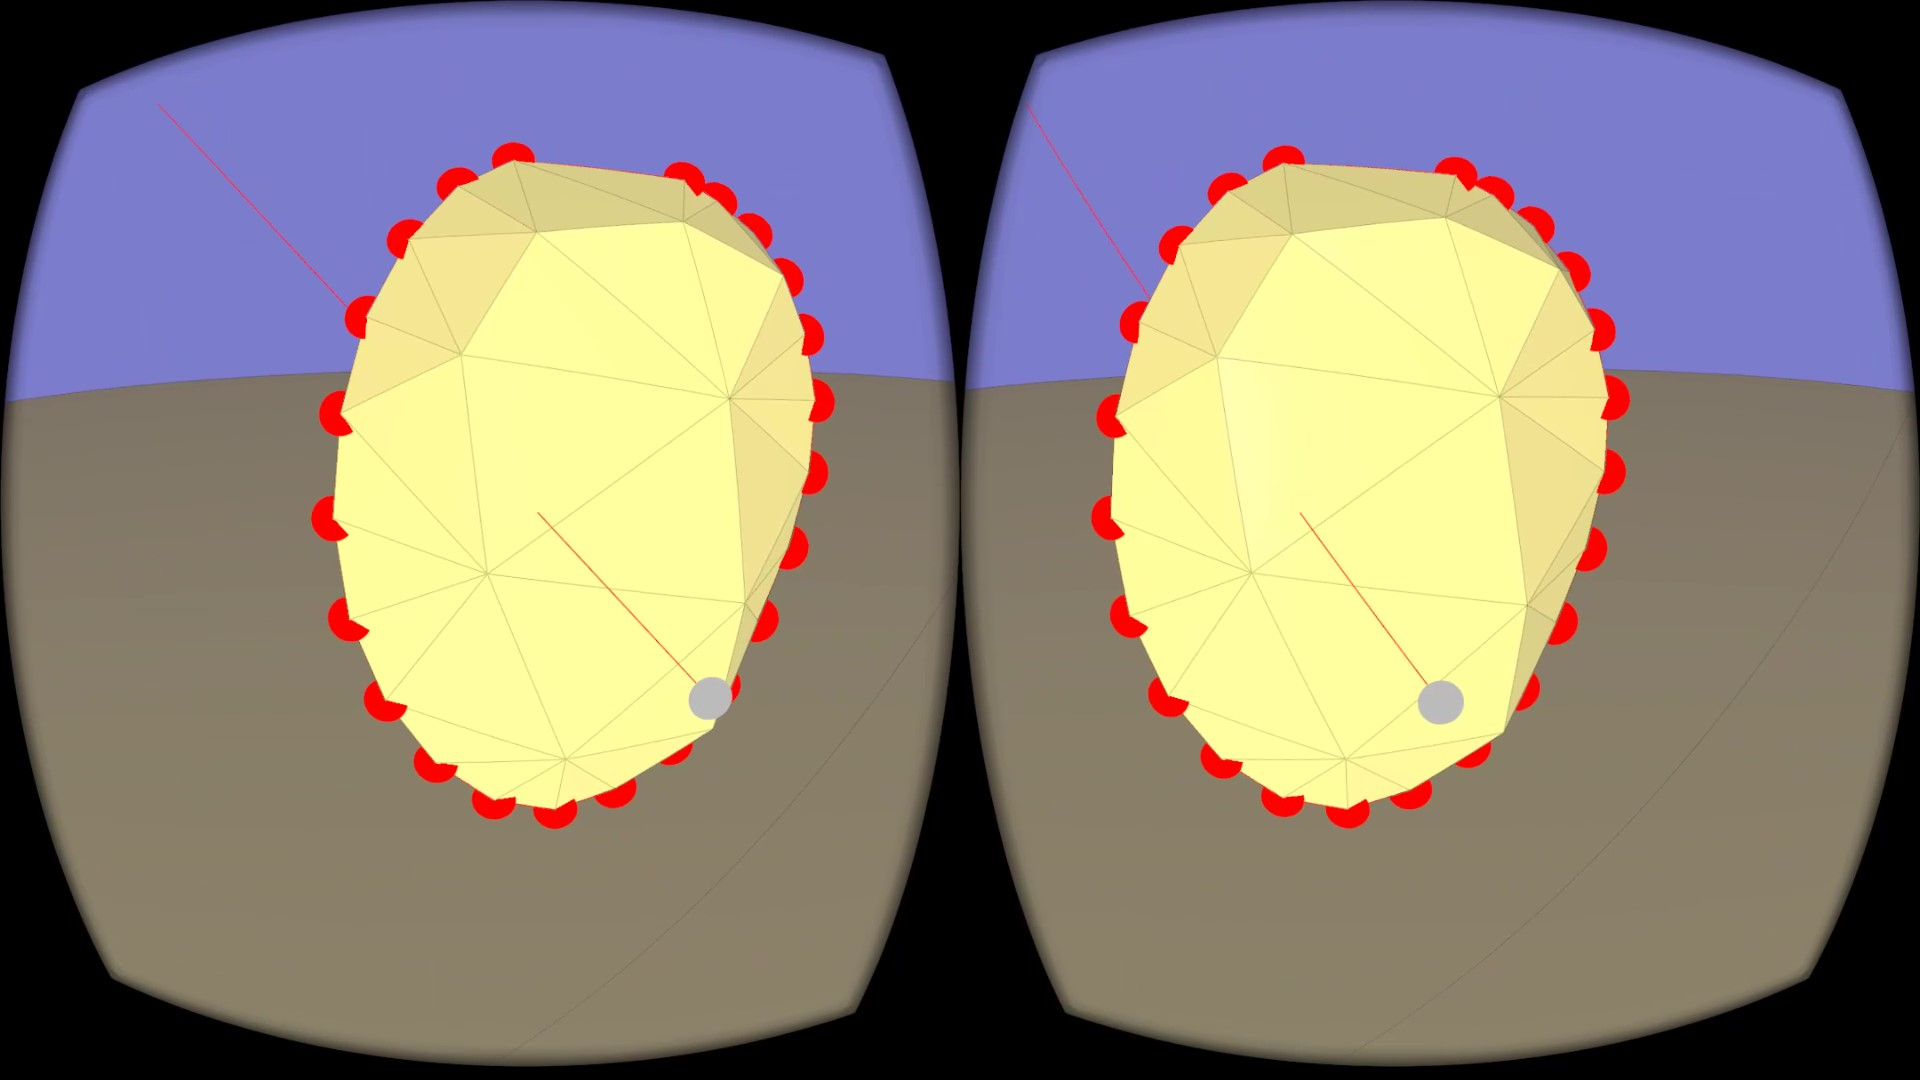
\includegraphics[width=0.45\linewidth]{figures/pre_extrude} &
       	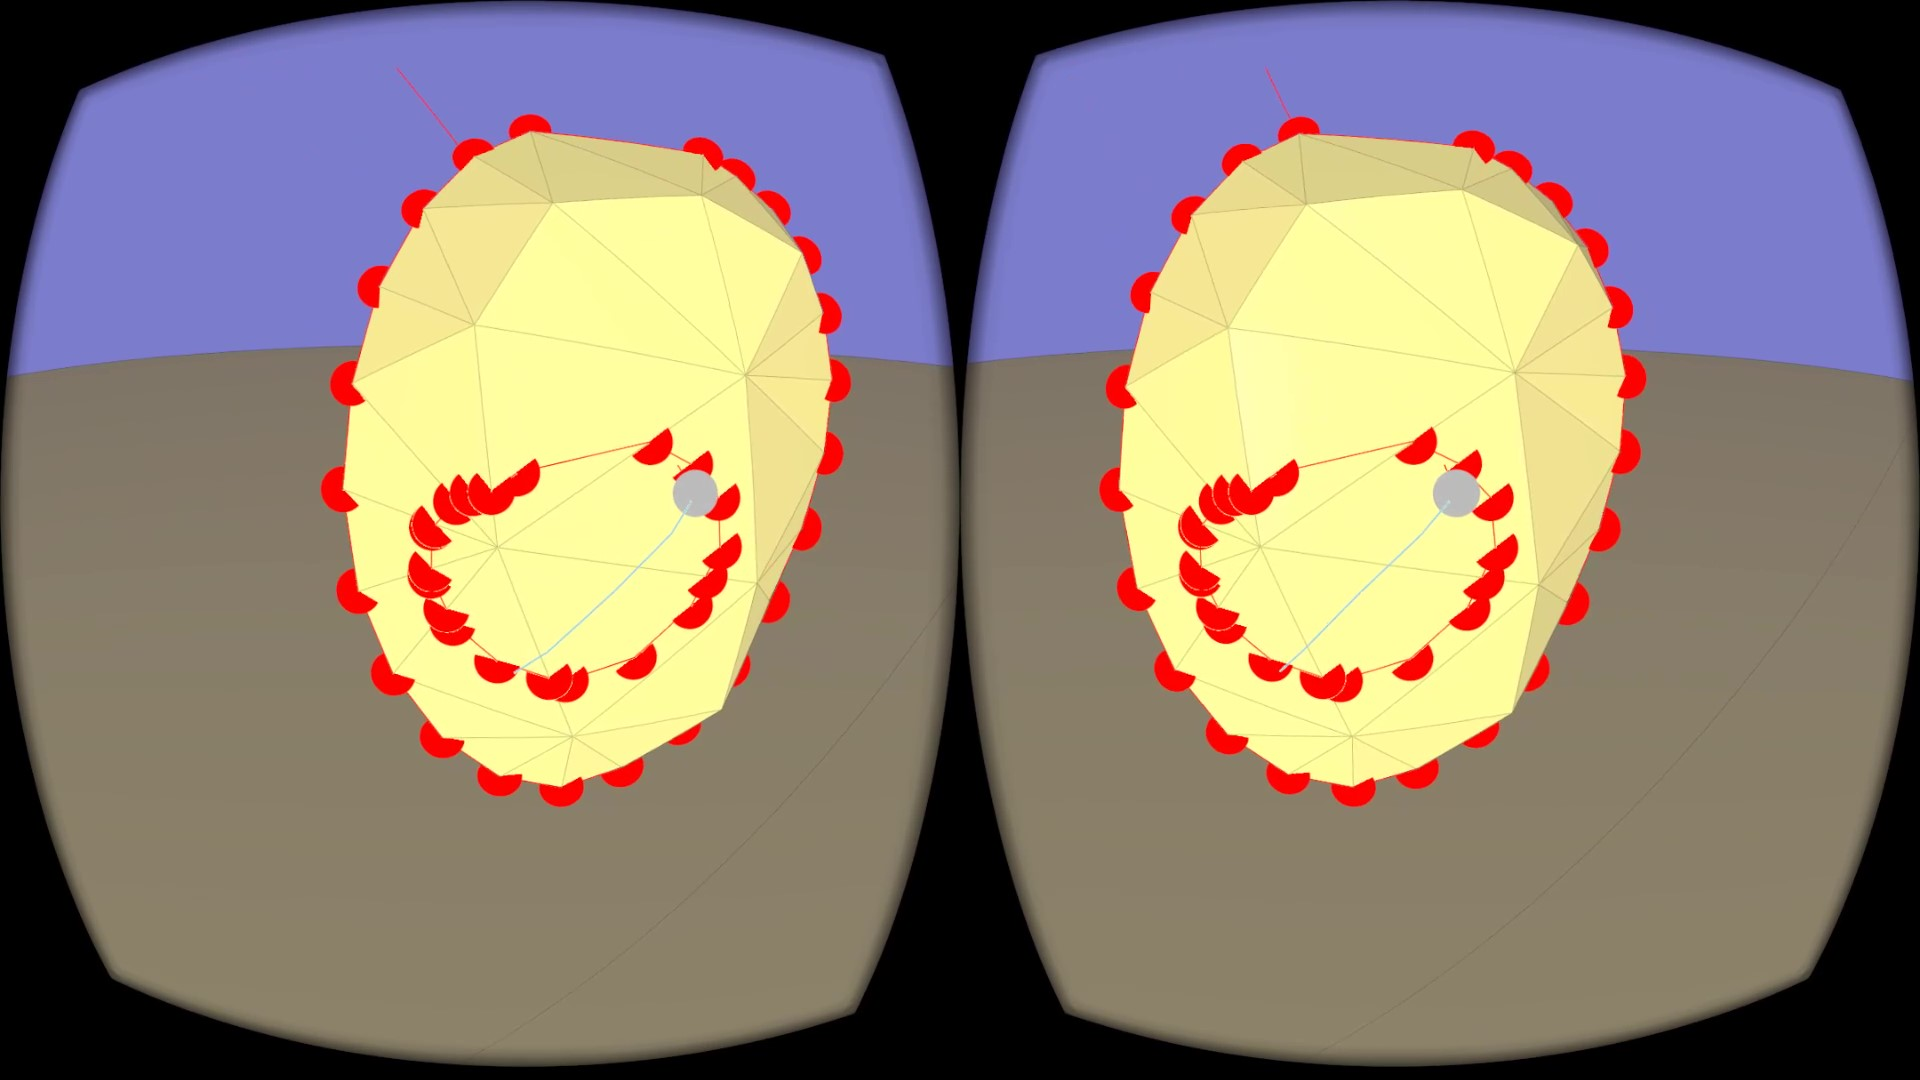
\includegraphics[width=0.45\linewidth]{figures/during_extrude2} \\
       	(a)&(b)\\
       	\end{tabular}
       	
       	  \centering
    \setlength{\tabcolsep}{0.0130\linewidth}
    \begin{tabular}{@{}c@{}}
    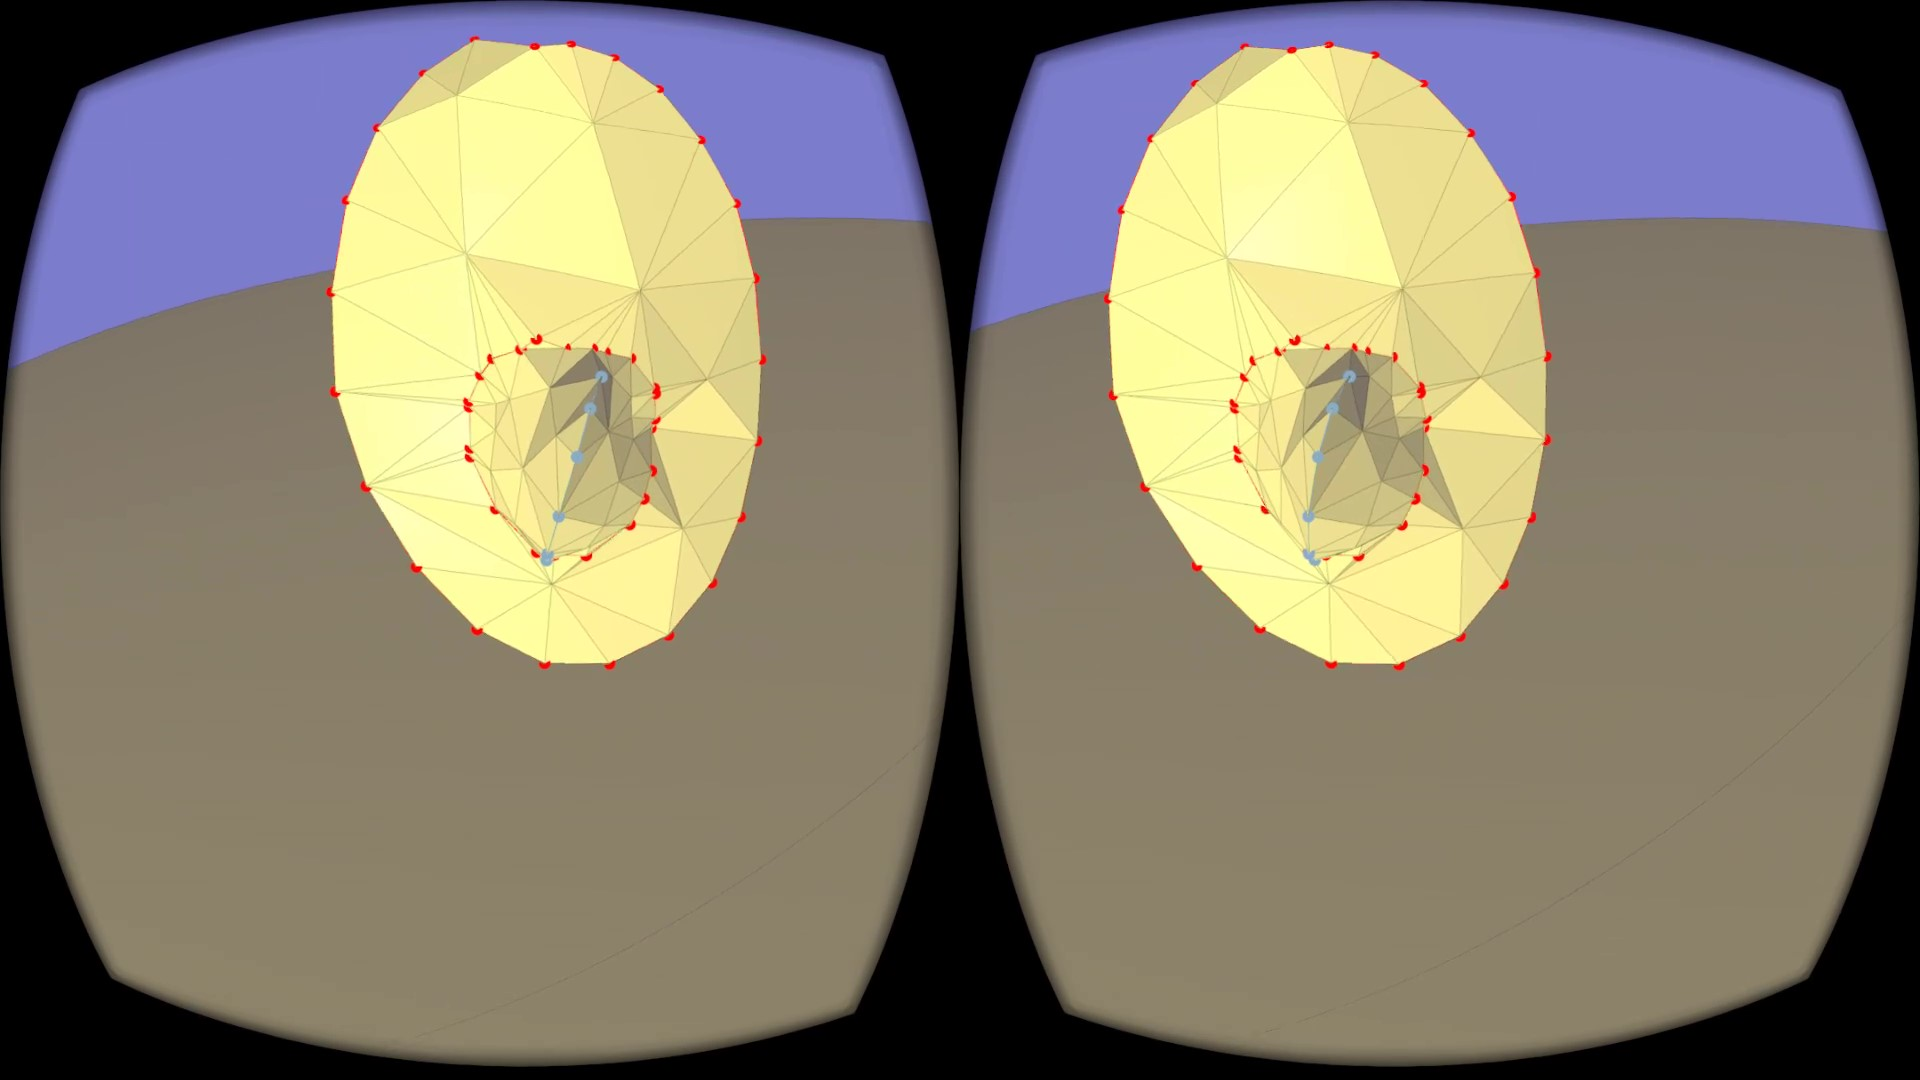
\includegraphics[width=0.926\linewidth]{figures/post_extrude}\\
    (c)
    \end{tabular}
    \caption[Extrusion action]{Extrusion action.
    	  \textup{(a)} Before \textup{(b)} During \textup{(c)} After
      \label{fig:extrude_example}}
\end{figure}

\begin{figure}[!h]
    \centering
    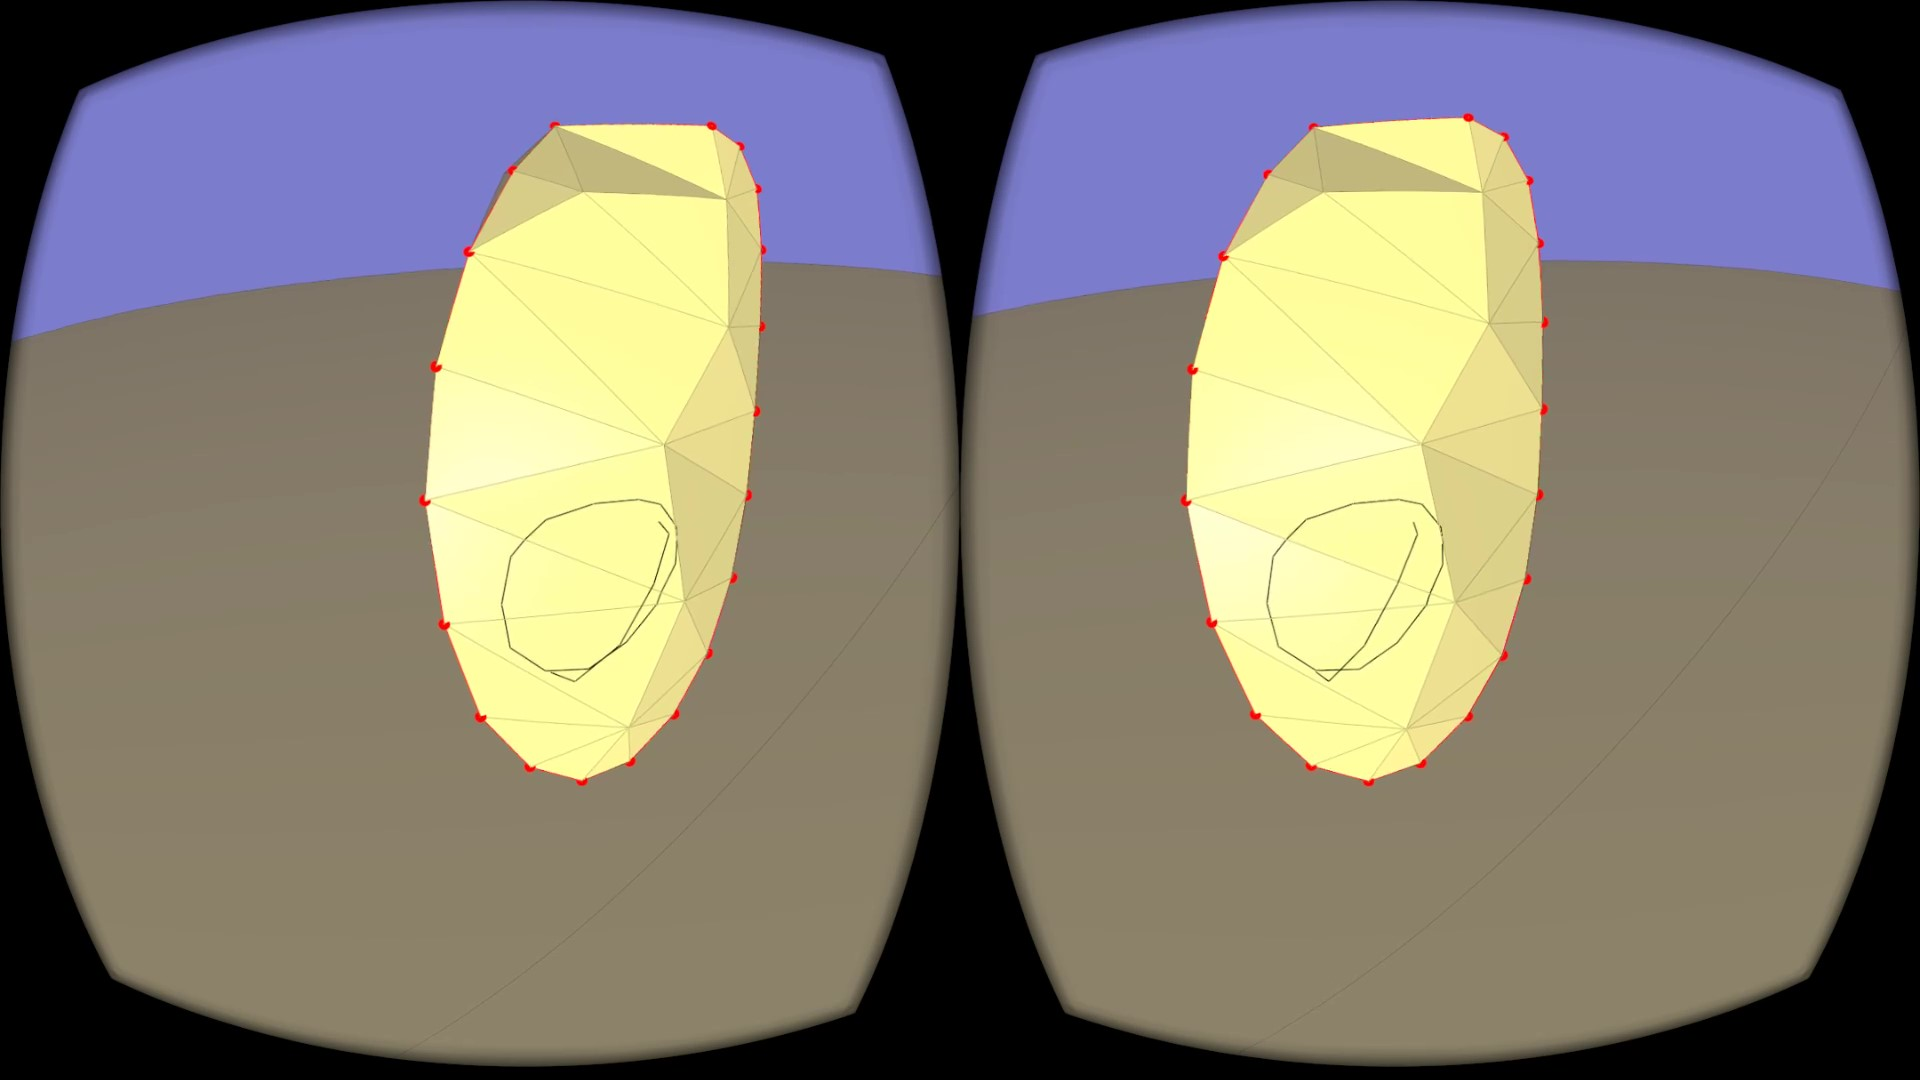
\includegraphics[width=0.7260\linewidth]{figures/error_extrusion}\\
    \caption[Error screen as result of a problematic extrusion]{Error screen as result of a problematic extrusion base stroke (it does not contain any vertex on its interior).
      \label{fig:errordisplay}}
\end{figure}

\subsection{Curve deformation}
Finally there are some changes in the way that curve deformation is handled when moving from non-VR to a VR setting. Whereas in the non-VR version of SketchMeshVR we project all vertices on the constraint curves to 2D in order to find the closest vertex to the 2D screen position of our mouse pointer, in SketchMeshVR we simply compare the 3D position of the Touch controller with the 3D positions of all selectable vertices (vertices that are part of a constraint curve). If the closest vertex is within our threshold distance, we select it as the deformation dragging handle. In the case that the vertex is further away than the threshold, we instead go into navigation mode in the non-VR case and in VR we simply ignore the action. Directly using the vertex 3D coordinates instead of projecting vertex positions to 2D avoids ambiguity when multiple 3D coordinates with different depth values result in the same screen coordinates. 

When determining where to move the selected handle vertex to, in non-VR we unproject the screen coordinates to a 3D coordinate using the z-value belonging to the projection of the deformation handle vertex, resulting in a displacement in the XY-plane. In VR on the other hand, we simply take the actual 3D position of the Touch controller. Figure~\ref{fig:pull_example} shows an example of an out-of-plane curve deformation.

\begin{figure}[!h]
    \centering
    \setlength{\tabcolsep}{0.0130\linewidth}
    \begin{tabular}{@{}cc@{}}
    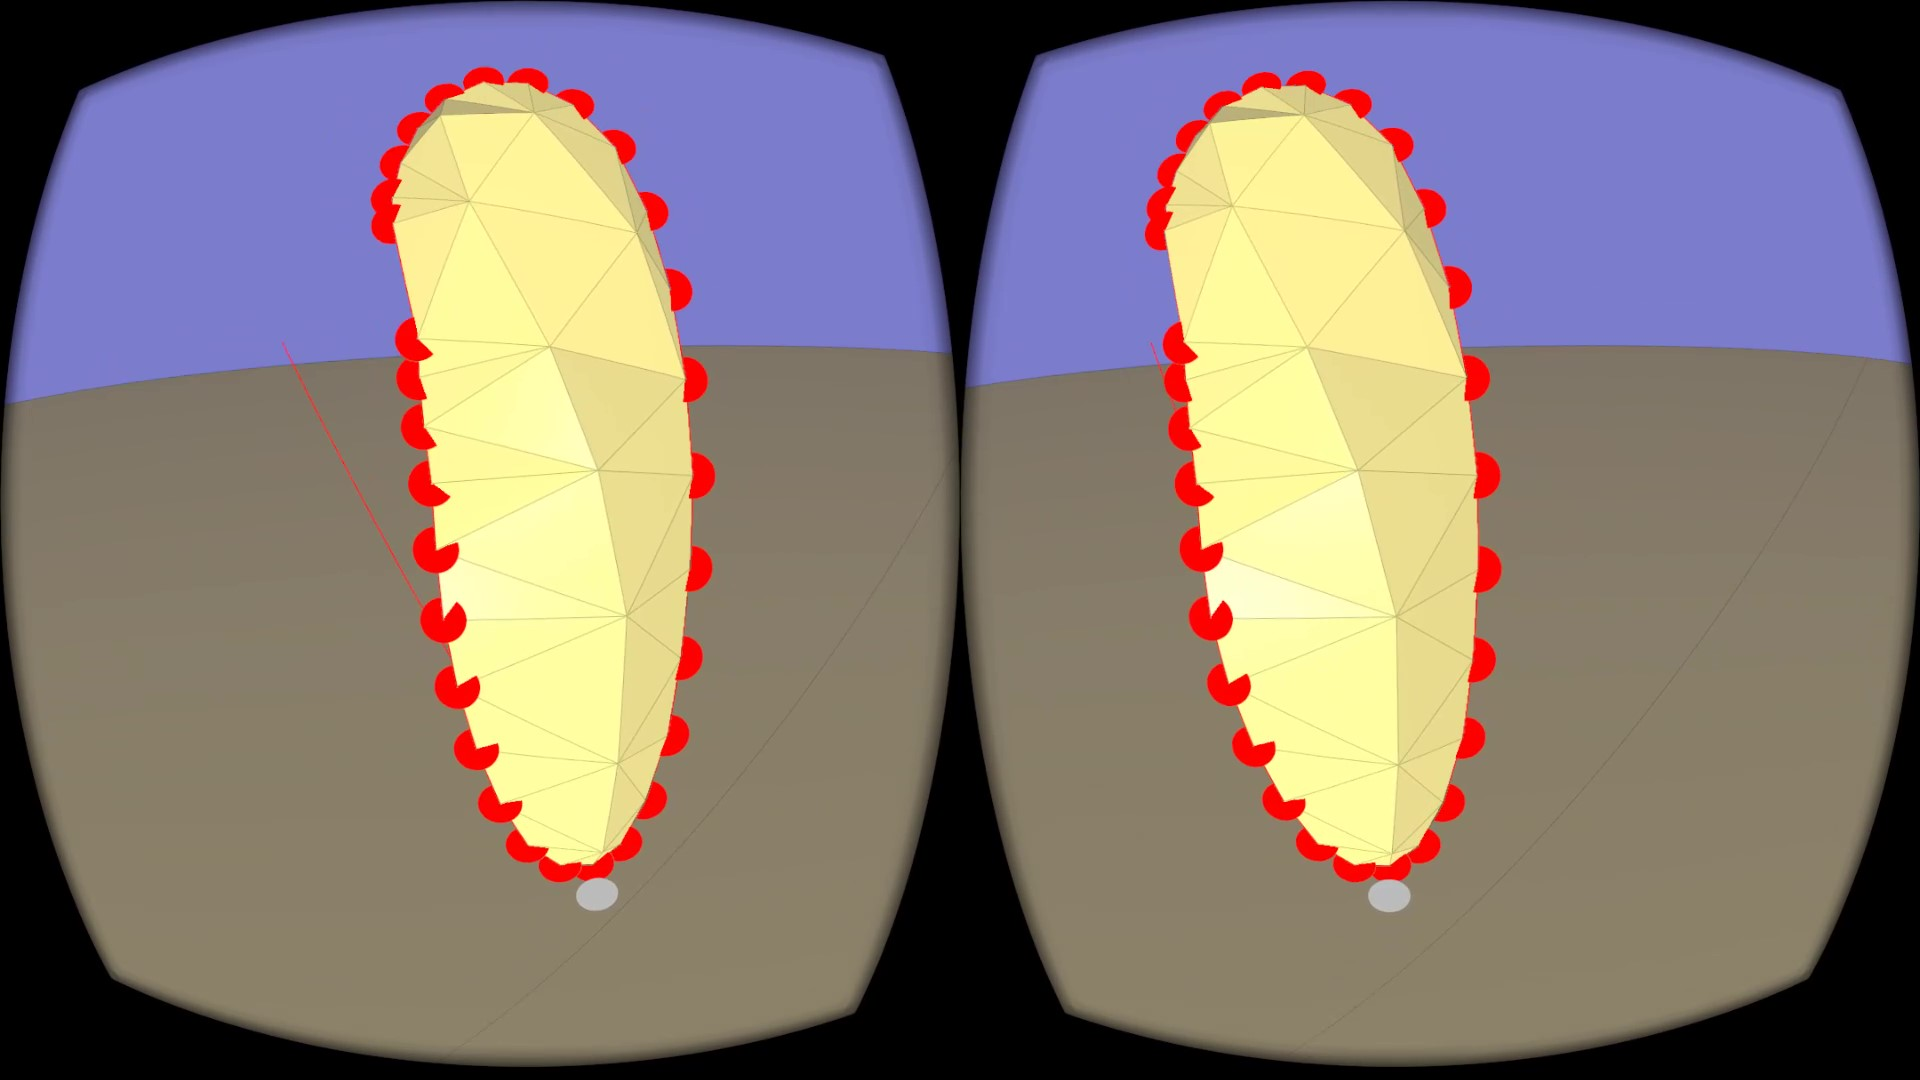
\includegraphics[width=0.45\linewidth]{figures/pre_pull} &
       	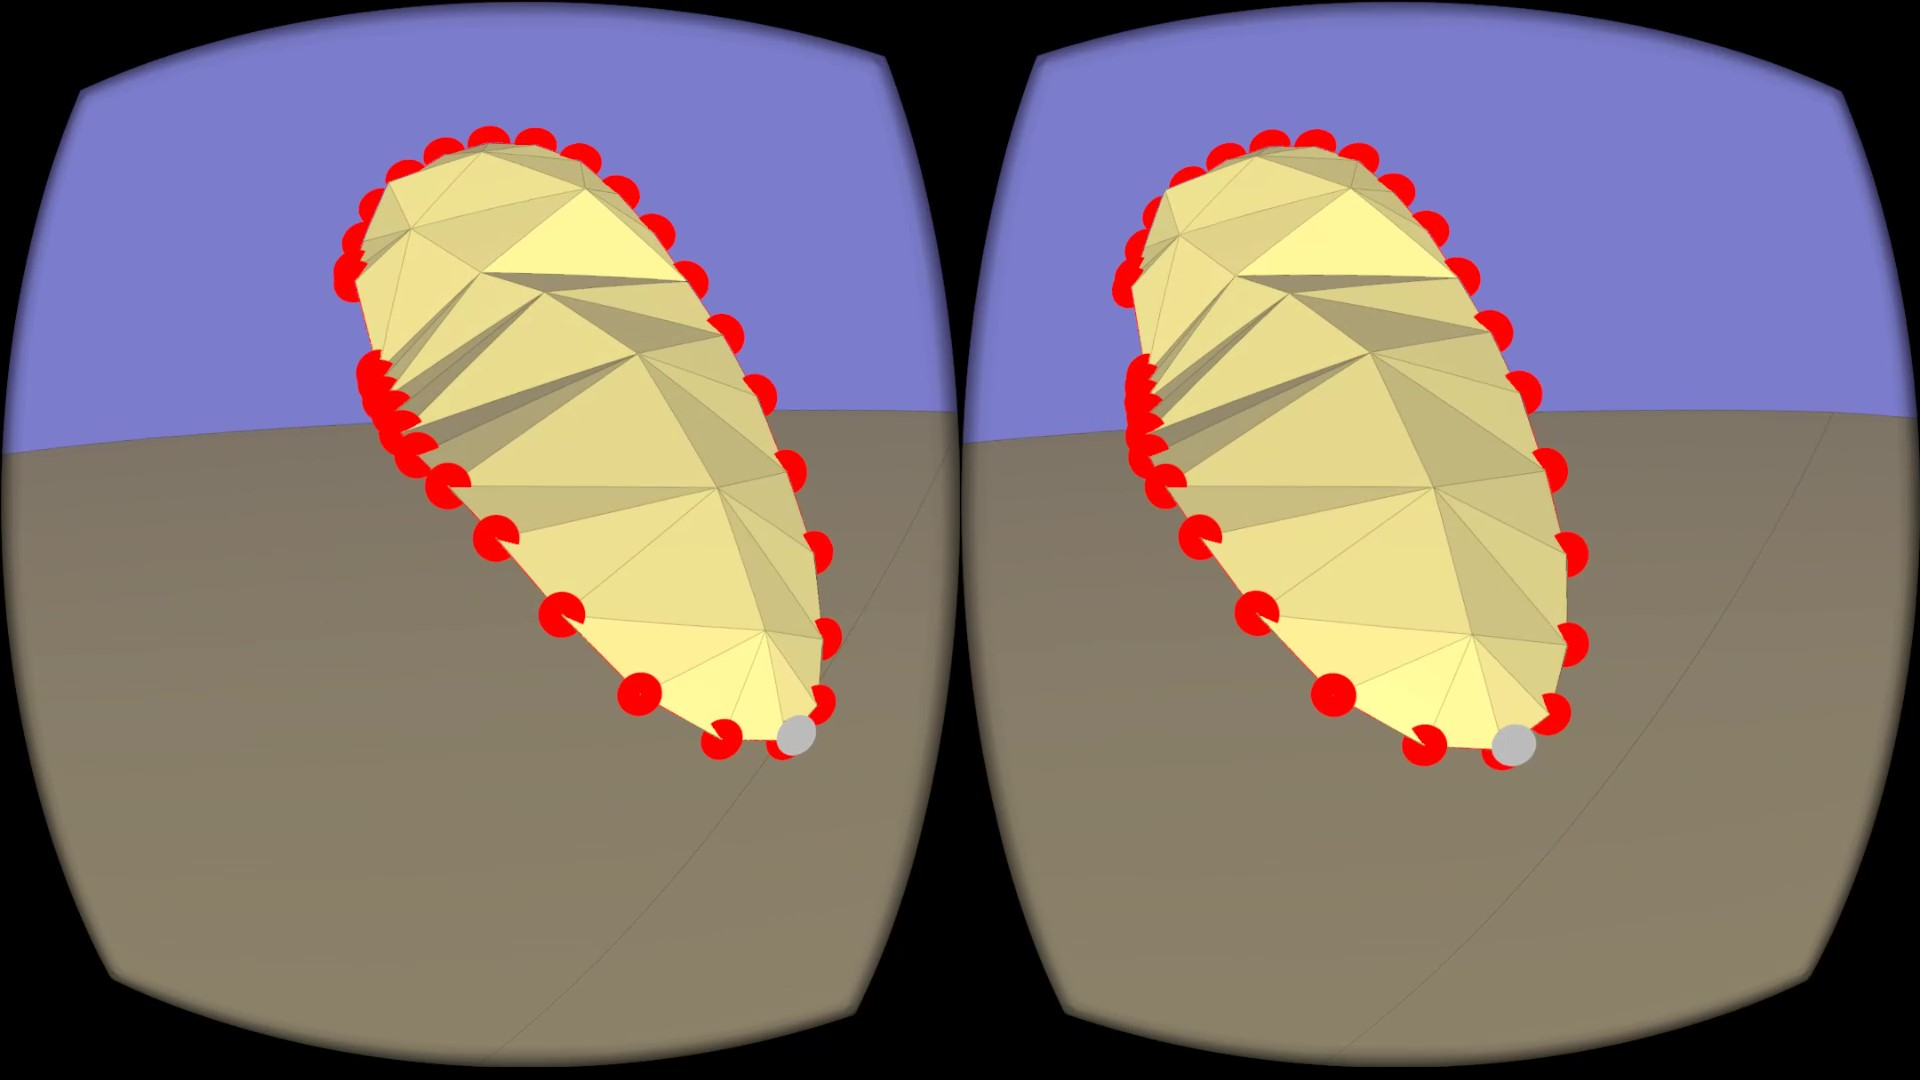
\includegraphics[width=0.45\linewidth]{figures/during_pull} \\
       	(a)&(b)\\
       	\end{tabular}
       	
       	  \centering
    \setlength{\tabcolsep}{0.0130\linewidth}
    \begin{tabular}{@{}c@{}}
    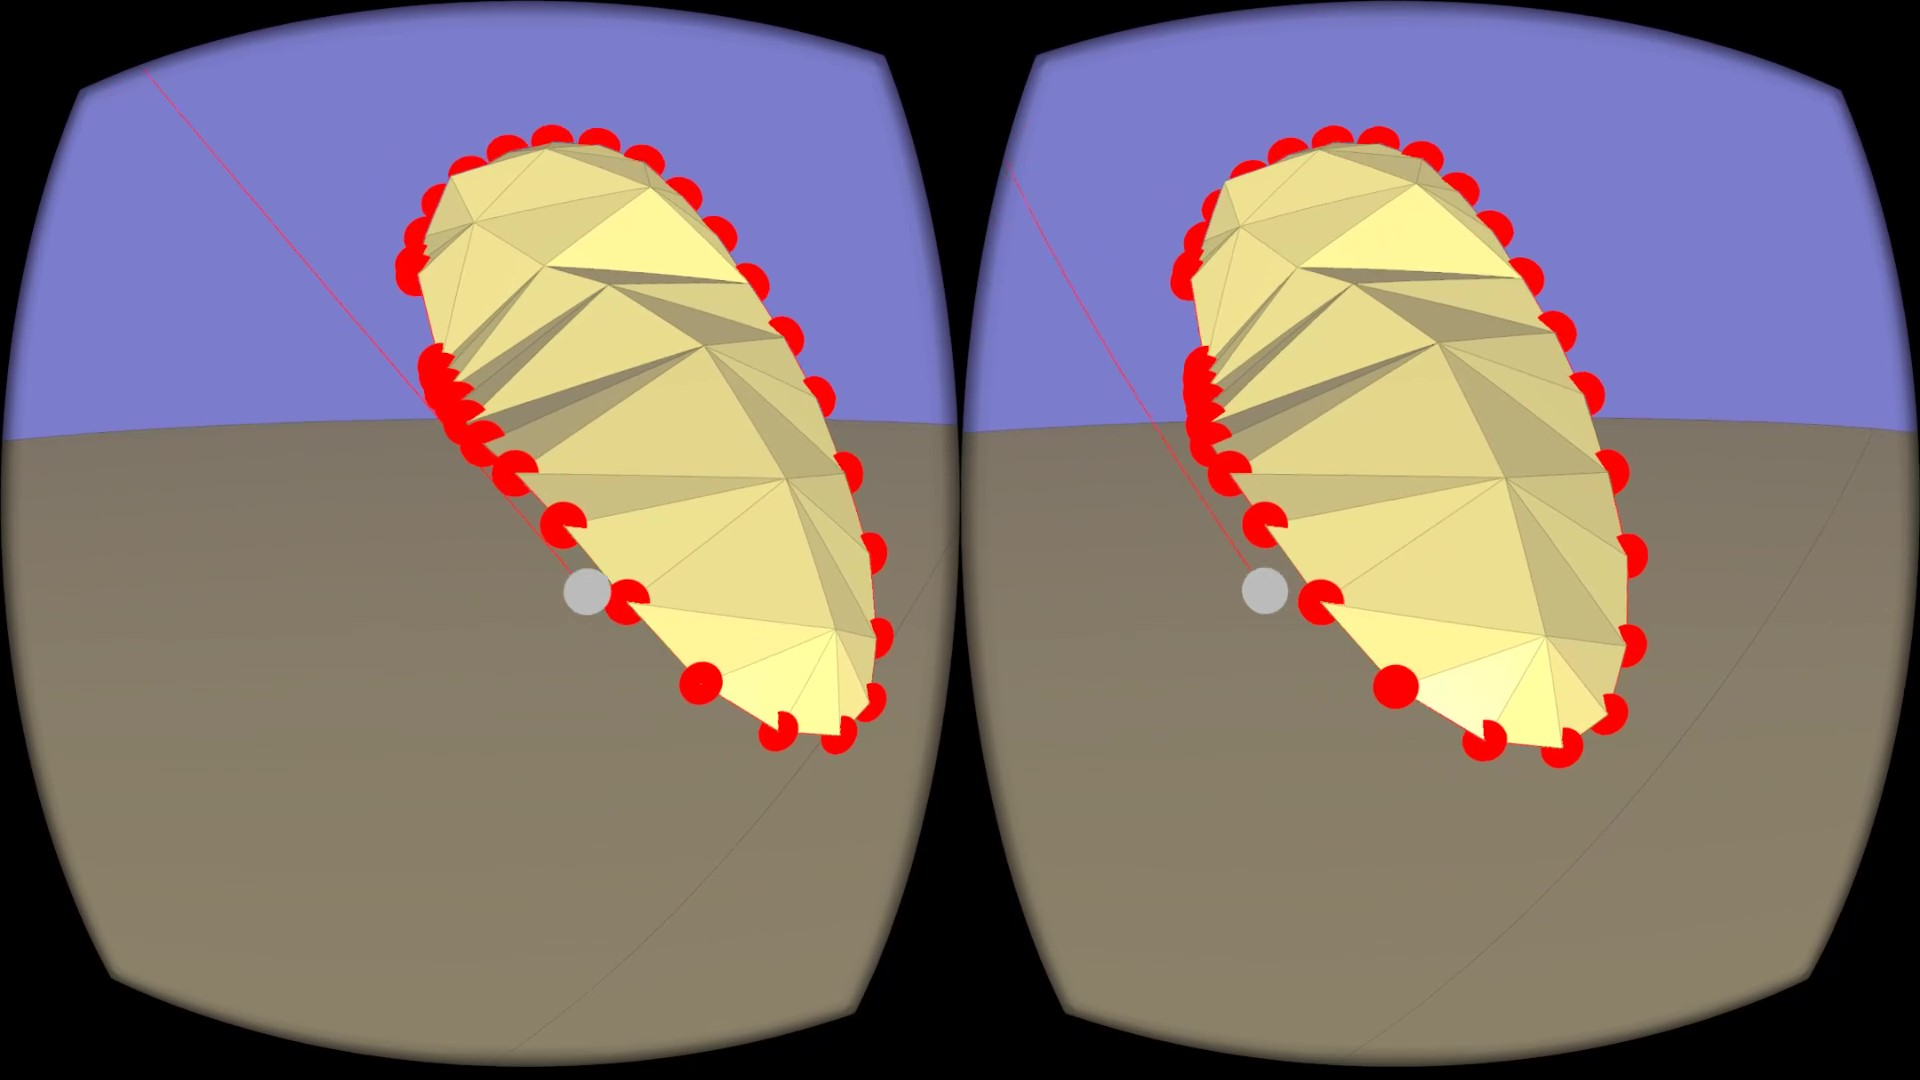
\includegraphics[width=0.926\linewidth]{figures/post_pull}\\
    (c)
    \end{tabular}
    \caption[Curve deformation action]{Curve deformation action.
    	  \textup{(a)} Before \textup{(b)} During \textup{(c)} After
      \label{fig:pull_example}}
\end{figure}

\section{User Interface}
For the user interface in virtual reality it was important to keep the controls for all actions very intuitive. Unlike the VR 3D modeling programs that were discussed in Section~\ref{sec:3dmodeling}, SketchMeshVR does not have any menus in its interface. Instead all functionality in the program can be used with just the right Touch controller (in future versions the user should be able to choose whether to use the left or right controller as the primary one). To increase spatial awareness and simplify orientating the user's hand in the scene, a sphere is displayed at the location of the right Touch controller, together with a ray from the hand following the orientation of the controller. When the user is in draw or pull mode or is drawing the extrusion silhouette, the ray disappears and only the hand sphere shows. This is done in order to emphasize that the actual position of the hand is used to draw a stroke, instead of the intersection points of the ray and mesh. Next to that we added a base floor to the scene, giving the user a reference point for orientation and minimizing the chance of motion sickness.

Compared to drawing strokes with a mouse on a PC screen (which happens purely in a 2D plane), drawing strokes in virtual reality with the Oculus Touch controller allows the user to draw strokes directly in 3D. In SketchMeshVR we made use of this advantage whenever possible. However, when the user draws the stroke that is used to create the initial mesh, the software does work best when the stroke is drawn mostly on the plane that the user is looking at. This is due to the fact that the drawn points will be projected to this 2D plane before they are triangulated, and thus it will result in a more regular mesh geometry if the drawn stroke lies mostly on the plane. For subsequent cutting or extrusion operations there is no benefit to drawing strokes in the plane that is being viewed, as for these actions the actual 3D positions of the drawn points are used. The rest of this section describes how to employ each of the editing modes from within our application.

\begin{figure}[!h]
    \centering
    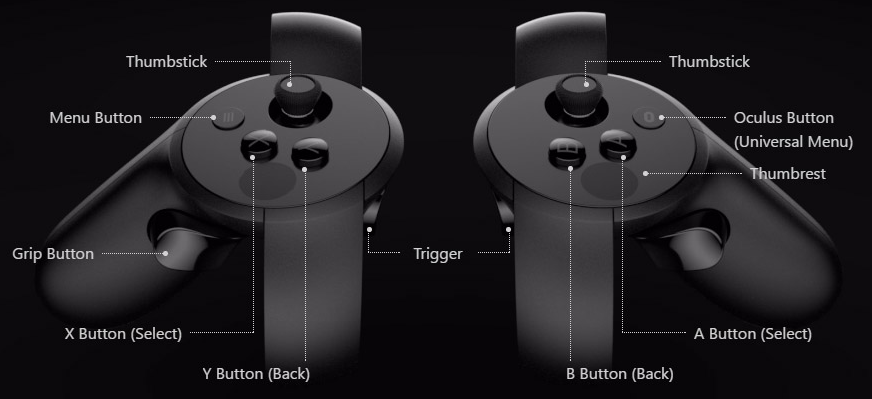
\includegraphics[width=0.7260\linewidth]{figures/touch_controllers}\\
    \caption[Oculus Touch controllers]{Button layout of the Oculus Touch controllers.
      \label{fig:touch_controller}}
\end{figure}

\begin{table}
    \centering
    \ra{1.1}
    \begin{tabular}{p{0.25\linewidth}p{0.25\linewidth}p{0.25\linewidth}}
    \toprule
    \emph{Action button} & \emph{Toggle button} & \emph{Actions}\\
    \midrule
		Grip & A button &Cut \& extrude\\
		Trigger  &B button &Add \& remove curves\\
		Grip + Trigger  &Thumbstick &Draw \& pull\\
    \bottomrule
    \end{tabular}
    \caption[Button mappings]{Button mappings for the different actions (the default action is mentioned first).\label{tab:buttonmap}}
\end{table}

\subsection{Drawing and mesh deformation}
To create an initial mesh, the user has to simultaneously press and hold the grip and trigger buttons while drawing a stroke in the 3D space and subsequently release both buttons when the stroke is finished. If the drawn stroke results in a non-edge manifold mesh (for example if the stroke intersects itself), a beep will sound and the stroke is displayed in black. Otherwise the created mesh will be shown, with the originally drawn stroke overlayed. 

In order to deform the mesh, a user can drag on all mesh constraint curves, which are indicated by a overlay that places coloured points on the vertices and coloured edges between them. The user can toggle between drawing and deformation mode by pressing the B button, with draw mode being selected upon startup. To perform the dragging, the user has to simultaneously press and hold down the grip and trigger buttons while his hand is close to the constraint vertex that he wants to pull to a new position. Then, while still pressing the grip and trigger buttons, the user needs to move his hand to the desired new position, and release both buttons when the desired result is achieved. The new vertex position is interpreted directly as the 3D position of the Touch controller, therefore also allowing deformation outside of the viewing plane (as compared to the non-VR version, which only allows in-plane deformation). 

The combination of grip and trigger buttons was chosen for these actions as they most resemble the feeling of holding a pencil and grabbing something in order to pull on it. 

\subsection{Adding and removing control curves}
To add extra control curves to an existing mesh, the user has to press and hold the trigger button while drawing the stroke onto the mesh. All points that are outside of the mesh will be ignored and will not be added to the control curve. 

In order to remove control curves (which is available on all constraint curves except for the curve that created the initial mesh), the user can toggle from stroke adding mode to stroke removal mode by pressing down the right thumbstick. Upon startup the stroke adding mode is selected. Whereas the drawing and deformation modes use the actual 3D position of the Touch controller, for adding and removing control curves the intersection between the hand ray and mesh are being used. 

We decided to map the trigger button to the functions of adding and removing control curves since this feels like a natural way to select objects (removal) and to highlight areas (addition).

\subsection{Cutting and extruding}
Finally with the A button the user can switch between cut and extrusion modes. Upon startup the toggle is set to cutting mode, which allows the user to cut parts of the existing mesh away. To make a cut the user has to first point the laser ray to somewhere outside of the mesh, and then while holding down the grip button draw the cutting stroke over the mesh and finally releasing somewhere outside of the mesh again. In order to minimize unwanted behaviour, cut strokes should be drawn at a pace that is not too fast. If anything went wrong during the cutting procedure, the drawn stroke will show on the mesh in black and a beep will sound. When looking in the direction the stroke was drawn in, the part of the mesh that is on the left hand side of the stroke will be removed.

When in extrusion mode, the user has to start drawing the stroke on the mesh and then while pressing the grip button has to draw the entire extrusion base on the mesh and release the button when the stroke is complete. Just like in the control curve addition mode, any points that are drawn outside of the mesh will be ignored. To ensure a correct functioning of the algorithm, the drawn base stroke needs to have at least one vertex on its interior. Then to complete the extrusion, the user has to draw the extrusion silhouette stroke that will define the height of the extrusion. When drawing this stroke, the user has to press and hold the grip button again but this time the actual position of the Touch controller will be used instead of the ray-mesh intersection point. Releasing the grip button will start the extrusion computations.

When pressing only the grip button, the hand often naturally assumes a position that resembles the way we symbolize pistols with our hands. Intuitively this maps to the concept of shooting a laser ray from your hand, which would be a sensible tool to cut a mesh with. For the case of extrusion we can argue something similar, as part of the mesh topology is also cut away. For this reason the grip button was mapped to the cut and extrude modes.